\documentclass[10pt, letterpaper, spanish]{book}

%----------- Useful packages --------------------------------

\usepackage[ansinew]{inputenc}
\usepackage[spanish]{babel}
\usepackage[intoc, spanish]{nomencl}
\usepackage{epstopdf}
\usepackage{makeidx}
%\usepackage{nomencl}
\usepackage[center]{caption}
\usepackage{titlesec}
\usepackage{cancel}
%
\let\counterwithout\relax
\let\counterwithin\relax
\usepackage{chngcntr}
%Math
\usepackage{amsthm, amssymb, amsmath, latexsym}
%Hyperlinks and colors
\usepackage{hyperref}
\usepackage[dvipsnames]{xcolor}
%
\usepackage{float}
% Figures and Draws
\usepackage{tikz,pgf}
 \usetikzlibrary{babel}
 \usetikzlibrary{arrows, positioning, intersections, shapes.arrows}
% Images
\usepackage{graphicx}
 \graphicspath{{Images/}}
% Bibliography
\usepackage{cite}

\usepackage{pdfpages}
\usepackage{fancyhdr}
 
 %--------- Margins and Format --------------------------
 
 \frenchspacing
\oddsidemargin = -10pt
\evensidemargin = -10pt
\headheight = 0pt      %%13pt 
\topmargin = 0pt       %%22pt
\headsep = 27pt        %%19pt
\textheight = 630pt
\textwidth = 500pt
\marginparsep = 7pt
\marginparwidth = 96pt
\paperheight=11in
\paperwidth=8.5in
\footskip = 27pt       %% 27pt
\hoffset = 0pt
\voffset = 0pt

%\pagestyle{fancy}

%---------- Other Settings ----------------------------------

\makenomenclature
\makeindex

\theoremstyle{definition}
\newtheorem{mydef}{Definici\'{o}n}[chapter]
\theoremstyle{plain}
\newtheorem{thm}[mydef]{Teorema}
\newtheorem{pro}[mydef]{Proposici\'{o}n}
\theoremstyle{remark}
\newtheorem{ex}{Ejemplo}
\newtheorem{obs}{Observaci\'{o}n}
\newtheoremstyle{break}
 {\topsep}{\topsep}
 {\normalfont}{}
 {\mdseries}{}
 {\newline}{}
\theoremstyle{break}
\newtheorem*{dem}{Demostraci\'{o}n:}

%---------- Renewed commands --------------------------------

%\renewcommand{\footnotemark}{\roman{footnotem}}

%---------- Begin Document ----------------------------------

\begin{document}

\printnomenclature
\tableofcontents{}

%-------------------------------------------------------------
% NOMENCLATURE
%-------------------------------------------------------------

%\nomenclature{$\mathbf{G}$}{Grupo}

%-------------------------------------------------------------
% INTRODUCTION
%-------------------------------------------------------------

\chapter*{Introducci\'{o}n}

La Relatividad General es la teor\'{i}a moderna de la gravedad, postulada por Albert Einstein a finales de 1915 \cite{Einstein}. En esta teor\'{i}a la gravedad no es una fuerza como los es en f\'{i}sica Newtoniana, sino la \emph{curvatura} del espacio-tiempo. Citando a John A. Wheeler ``la materia le dice al espacio-tiempo c\'{o}mo curvarse, y el espacio-tiempo le dice a la materia c\'{o}mo moverse''. {\color{OliveGreen} hablar un poco m\'{a}s de la relatividad general, contar sobre sus predicciones y sus l\'{i}mites y as\'{i} poder argumentar por qu\'{e} surge el formalismo de variables de Ashtekar.}

En \'{e}sta tesis supondremos que el lector est\'{a} familiarizado con la teor\'{i}a de Relatividad General y conceptos b\'{a}sicos de Geometr\'{i}a Diferencial.

El prop\'{o}sito de esta tesis es encontrar la forma que toman las Variables de Conexi\'{o}n para los casos de cosmolog\'{i}as homogeneas e isotr\'{o}picas. Para ello, es importante entender las distintas formulaciones de la Relatividad General, principalmente en la formulaci\'{o}n de variables de conexi\'{o}n hecha por A. Ashtekar \cite{Ashtekar86, Ashtekar87}. En el primer cap\'{i}tulo se presentar\'{a} la formulaci\'{o}n Lagrangiana y Hamiltoniana de la Relatividad General (siguiendo de cerca la discusi\'{o}n que se lleva acabo en \cite{Poisson}). En el segundo veremos la formulaci\'{o}n en variables de conexi\'{o}n de la Relatividad General, tomando como principales referencias el libro de J. C. Baez \cite{Baez}, el art\'{i}culo de J. Barbero \cite{Barbero} y la tesis de J. Vega \cite{Vega}. Y en el tercer cap\'{i}tulo presentamos como obtener la forma de las variables de conexi\'{o}n para espacios homog\'{e}neos e isotr\'{o}picos tomando como base el art\'{i}culo de Bojowald \cite{Bojowald2005}, pero apoy\'{a}ndonos en gran parte en el trabajo hecho por S. Kobayashi y K. Nomizu en su libro \cite{Kobayashi} y el art\'{i}culo sobre clasificaci\'{o}n de haces sim\'{e}trico y conexiones de O. Brodbeck \cite{Brodbeck}.

En esta tesis usaremos la convenci\'{o}n de signos de Misner, Thorne, y Wheeler con una m\'{e}trica de signatura $(-,+,+,+)$. Los \'{i}ndices griegos $\alpha$, $\beta...$ ser\'{a}n utilizados para las componentes espacio-temporales, es decir, corren de 0 a 3; los \'{i}ndices latinos $a$, $b$, $c...$ corren de 1 a 3, est\'{a}n asignados para las componentes espaciales; las letras latinas may\'{u}sculas $I$, $J$, $K$..., ser\'{a}n usadas para los \'{i}ndices internos.

%-------------------------------------------------------------
% LAGRANGIAN FORMULATION GENERAL RELATIVITY
%-------------------------------------------------------------

\chapter{Formulaci\'{o}n Lagrangiana y Hamiltoniana de la Relatividad General}
\label{chp:RG}

%-------------------------------------------------------------
% LAGRANGIAN FORMULATION
%-------------------------------------------------------------

\section{Formulación Lagrangiana}
\label{sec:FL}

En la formulación Lagrangiana de la Relatividad General, el funcional de acción $S$ está definido como la integral de una densidad lagrangiana sobre una región 4-dimensional $\Omega$, de una variedad diferenciable $\mathcal{M}$ con la topología del espacio-tiempo, delimitada por una hipersuperficie cerrada $\partial \Omega$.  Dicho funcional de acción $S$ está formado por dos partes, la asociada al campo gravitacional $g_{\mu \nu}$, es decir la geometría, denotado por $S_{G}[g]$ y la parte correspondiente a los campos de materia, $S_{M}[\phi; g]$, esto es
%
\begin{equation}
\label{eq:S}
S[g; \phi] = S_{G}[g] + S_{M}[\phi; g].
\end{equation}

El campo dinámico es la métrica del espacio-tiempo $g_{\mu \nu}$, cuyas componentes dependen de las coordenadas $x^{\alpha}$ en la región $\Omega$. Así, para obtener las ecuaciones de campo gravitacional vía el Principio de Mínima Acción, se introduce la variación arbitraria $\delta g_{\mu \nu}(x^{\alpha})$ en $\Omega$ con la condición de que dicha variación sea nula en la frontera $\partial \Omega$,
%
\begin{equation}
\label{eq:boundcond}
\delta g_{\mu \nu} \Big|_{\partial \Omega} = 0.
\end{equation}
Esto quiere decir que la métrica inducida\footnotemark $h_{\alpha \beta}$ en la hipersuperficie $\partial \Omega$ se mantiene fija.
\footnotetext{La forma fundamental de la métrica inducida en $\partial \Omega$ es $h_{\alpha \beta} = g_{\mu \nu} \frac{\partial x^{\mu}}{\partial y^{\alpha}} \frac{\partial x^{\nu}}{\partial y^{\beta}} = g_{\mu \nu} e^{\mu}_{\alpha} e^{\nu}_{\beta}$, donde $e^{\mu}_{\alpha}=\frac{\partial x^{\mu}}{\partial y^{\alpha}}$.} 

El funcional de acción del campo de materia, $S_{M}$, está dada por
%
\begin{equation}
\label{eq:SM}
S_{M} [\phi; g] = \int_{\Omega} \mathcal{L}(\phi, \partial_{\alpha} \phi; g, \partial_{\alpha} g_{\mu \nu}) \sqrt{-g} \, d^{4} x.
\end{equation}
%
Por otro lado, la parte gravitacional de la acción $S_{G}[g]$, para facilitar los cálculos, se divide en tres términos; a saber,
%
\begin{equation}
\label{eq:SG}
S_{G}[g] = \frac{1}{16 \pi} (I_{EH}[g] + 2 I_{B}[g] + 2 I_{0}),
\end{equation}
%
el término de Einstein-Hilbert $I_{EH}[g]$, un término de frontera $I_{B}[g]$ y un término no dinámico $I_{0}$, que únicamente influye en el valor numérico de la acción mas no en las ecuaciones de movimiento, donde
%
\begin{equation*}
I_{EH}[g] = \int_{\Omega} R \sqrt{-g} \, d^{4} x, \quad I_{B}[g] = \oint_{\partial \Omega} \varepsilon K \sqrt{|h|} d^{3} y, \quad I_{0}[g] = \oint_{\partial \Omega} \varepsilon K_{0} \sqrt{|h|} d^{3} y \, .
\end{equation*}
%
Aquí, las coordenadas $x^{\mu}$ se utilizarán en $\Omega$ mientras que las coordenadas $y^{\alpha}$ en $\partial \Omega$. $R$ es el escalar de Ricci, $g$ es el determinante de la métrica $g_{\mu \nu}$, $h$ es el determinante de la métrica inducida $h_{\alpha \beta}$ y $\varepsilon \equiv n^{\mu} n_{\mu} = \pm 1$ es el módulo del normal unitario\footnotemark  $n_{\mu}$ a $\partial \Omega$. $K$ es la traza de la curvatura extrínseca $K_{\alpha \beta}$ de $\partial \Omega$ y $K_{0}$ es la traza de la curvatura extrínseca de $\partial \Omega$ encajada en el espacio-tiempo plano.
\footnotetext{El módulo $\varepsilon$  de $n_{\mu}$ es $+1$ donde $\partial \Omega$ es tipo-tiempo y $-1$ donde es tipo-espacio.}

Al variar la acción $S[g; \phi]$ con respecto a $g_{\mu \nu}$, usando el hecho de que $\delta g = g g^{\mu \nu} \delta g_{\mu \nu}$ y $g^{\mu \nu} \delta g_{\mu \nu} = -g_{\mu \nu} \delta g^{\mu \nu}$, se obtiene, primero para la parte asociada a materia, que
%
\begin{align}
\label{eq:varSML}
\delta S_{M} & = \int_{\Omega} \delta (\mathcal{L} \sqrt{-g}) \, d^{4} x \nonumber \\
& = \int_{\Omega} \left( \frac{\partial \mathcal{L}}{\partial g^{\mu \nu}} \delta g^{\mu \nu} \sqrt{-g} + \mathcal{L} \delta \sqrt{-g} \right) \, d^{4} x \nonumber \\
& = \int_{\Omega} \left( \frac{\partial \mathcal{L}}{\partial g^{\mu \nu}} - \frac{1}{2} \mathcal{L} g_{\mu \nu} \right) \delta g^{\mu \nu} \sqrt{-g} \, d^{4} x \nonumber \\
& = - \frac{1}{2} \int_{\Omega} T_{\mu \nu} \delta g^{\mu \nu} \sqrt{-g} \, d^{4} x,
\end{align}
%
definiendo el tensor de energía-momento como
%
\begin{equation}
\label{eq:TabL}
T_{\mu \nu} := \mathcal{L} g_{\mu \nu} - 2 \frac{\partial \mathcal{L}}{\partial g^{\mu \nu}}.
\end{equation}
%
%se puede reescribir \eqref{eq:varSML} y así la variación de la acción correspondiente al campo de materia queda de la siguiente manera,
%
%\begin{equation}
%\label{eq:varSMT}
%\delta S_{M} = - \frac{1}{2} \int_{\Omega} T_{\mu \nu} \delta g^{\mu \nu} \sqrt{-g} \, d^{4} x.
%\end{equation}
%
Mientras que, para la parte correspondiente a la parte gravitacional $S_{G}[g]$, comenzando con el término de Einstein-Hilbert $I_{EH}$, se tiene que
%
\begin{align}
\label{eq:IEH}
\delta I_{EH} & = \int_{\Omega} \delta(R \sqrt{-g}) \, d^{4} x \nonumber \\
%& = \int_{\Omega} \delta(g^{\mu \nu} R_{\mu \nu} \sqrt{-g}) \, d^{4} x \nonumber \\
& = \int_{\Omega} (\delta g^{\mu \nu}) R_{\mu \nu} \sqrt{-g} \, d^{4} x + \int_{\Omega} g^{\mu \nu} (\delta R_{\mu \nu}) \sqrt{-g} \, d^{4} x + \int_{\Omega} g^{\mu \nu} R_{\mu \nu} (\delta \sqrt{-g}) \, d^{4} x \nonumber \\
& = \int_{\Omega} R_{\mu \nu} (\delta g^{\mu \nu}) \sqrt{-g} \, d^{4} x + \int_{\Omega} g^{\mu \nu} (\delta R_{\mu \nu}) \sqrt{-g} \, d^{4} x -  \int_{\Omega} \frac{1}{2} R \sqrt{-g} g_{\mu \nu} \delta g^{\mu \nu} \, d^{4} x.
\end{align}

Ahora bien, considerando un marco de referencia inercial local donde los símbolos de Christoffel sean cero, lo que implica que $\partial_{\sigma} = \nabla_{\sigma}$, entonces,
%
\begin{equation}
\label{eq:varRicci}
\delta R_{\mu \nu} = \partial_{\lambda} \delta \Gamma^{\lambda}_{\mu \nu} - \partial_{\nu} \delta \Gamma^{\lambda}_{\mu \lambda} = \nabla_{\lambda} \delta \Gamma^{\lambda}_{\mu \nu} - \nabla_{\nu} \delta \Gamma^{\lambda}_{\mu \lambda}.
\end{equation}
%
Tomando en cuenta que $\nabla_{\sigma} g^{\mu \nu} = 0$, al multiplicar \eqref{eq:varRicci} por $g^{\mu \nu}$ se tiene que
%
\begin{equation}
\label{eq:varSRicci}
g^{\mu \nu} \delta R_{\mu \nu} = g^{\mu \nu} \nabla_{\lambda} \delta \Gamma^{\lambda}_{\mu \nu} - g^{\mu \nu}\nabla_{\nu} \delta \Gamma^{\lambda}_{\mu \lambda}  = \nabla_{\lambda}(g^{\mu \nu} \delta \Gamma^{\lambda}_{\mu \nu} - g^{\mu \lambda} \Gamma^{\nu}_{\mu \nu}),
\end{equation}
%
y definiendo
%
\begin{equation}
\label{eq:v}
v^{\lambda} := g^{\mu \nu} \delta \Gamma^{\lambda}_{\mu \nu} - g^{\mu \lambda} \delta \Gamma^{\nu}_{\mu \nu},
\end{equation}
la expresión \eqref{eq:varSRicci} se reescribe como $g^{\alpha \beta} \delta R_{\alpha \beta} = \nabla_{\lambda} v^{\lambda}$. Aplicando el teorema de Gauss se obtiene
%
\begin{equation}
\label{eq:intDv}
\int_{\Omega} g^{\mu \nu} \left(  \delta R_{\mu \nu} \right) \sqrt{-g} d^4 x = \int_{\Omega} \nabla_{\mu} v^{\mu} \sqrt{-g} d^4 x = \oint_{\partial \Omega} \varepsilon v^{\mu} n_{\mu} \sqrt{|h|} d^3 y \, .
\end{equation}
%
Recordando la condición de frontera \eqref{eq:boundcond}, la variación de los símbolos de Christoffel en $\partial \Omega$ es
%
\begin{equation}
\label{eq:varGamma}
\delta \Gamma^{\sigma}_{\mu \nu} = \frac{1}{2} g^{\sigma \lambda} (\partial_{\mu} \delta g_{\nu \lambda} + \partial_{\nu} \delta g_{\lambda \mu} - \partial_{\lambda} \delta g_{\mu \nu}),
\end{equation}
%
entonces sustituyendo \eqref{eq:varGamma} en \eqref{eq:v} se llega a que
%
\begin{align}
\label{eq:vn}
n^{\lambda} v_{\lambda} \Big|_{\partial \Omega} & = n^{\lambda} g^{\mu \nu} (\partial_{\mu} \delta g_{\lambda \nu} - \partial_{\lambda} \delta g_{\mu \nu}) \nonumber \\
& = n^{\lambda} (\varepsilon n^{\mu} n^{\nu} + h^{\mu \nu}) (\partial_{\mu} \delta g_{\lambda \nu} - \partial_{\lambda} \delta g_{\mu \nu}) \nonumber \\
& = n^{\lambda} h^{\mu \nu} (\partial_{\mu} \delta g_{\lambda \nu} - \partial_{\lambda} \delta g_{\mu \nu}).
\end{align}
%
En \eqref{eq:vn} se uso la relación de completez $g^{\mu \nu} = \varepsilon n^{\mu} n^{\nu} + h^{\mu \nu}$. Ahora, por la condición de frontera \eqref{eq:boundcond}, las derivadas tangentes $e^{\alpha}_{\beta} \partial_{\alpha} \delta g_{\mu \nu}$ a $\partial \Omega$ deben anularse, sin embargo las derivadas normales de $\delta g_{\mu \nu}$ en $\partial \Omega$ no necesariamente se anulan, por lo que

\begin{equation}
\label{eq:vnh}
n^{\mu} v_{\mu} = - n^{\mu} h^{\alpha \beta} \partial_{\mu} \delta g_{\alpha \beta}.
\end{equation}
%
Reemplazando \eqref{eq:vnh} en \eqref{eq:intDv}, se llega a
%
\begin{equation}
\label{eq:intvnh}
\int_{\Omega} g^{\mu \nu} (\delta R_{\mu \nu}) \sqrt{-g} d^4 x = - \oint_{\partial \Omega} \varepsilon n^{\mu} h^{\alpha \beta} \partial_{\mu} \delta g_{\alpha \beta} \sqrt{|h|} \, d^{3} y,
\end{equation}
%
y finalmente, sustituyendo \eqref{eq:intvnh} en \eqref{eq:IEH} se obtiene que la variación del término de Einstein-Hilbert $I_{EH}$ está dada por
%
\begin{equation}
\label{eq:varIEH}
\delta I_{EH} = \int_{\Omega} \left(R_{\mu \nu} - \frac{1}{2} R g_{\mu \nu} \right) \sqrt{-g} \delta g^{\mu \nu} \, d^{4} x - \oint_{\partial \Omega} \varepsilon n^{\mu} h^{\alpha \beta} \partial_{\mu} \delta g_{\alpha \beta} \sqrt{|h|} \, d^{3} y.
\end{equation}

Ahora se hace la variación de $I_{B}$. Nótese que la única cantidad que varía es la traza de la curvatura extrínseca, i.e. $K$, pues la métrica inducida en $\partial \Omega$ se mantiene fija, es decir, $\delta \sqrt{|h|} = 0$, así que sólo es necesario calcular la variación de $K$ en $\partial \Omega$. Puesto que,
%
\begin{align}
\label{eq:definitionK}
K & = \nabla_{\mu} n^{\mu} = (\varepsilon n^{\mu} n^{\nu} + h^{\mu \nu}) \nabla_{\mu} n_{\nu} \nonumber \\
& = h^{\mu \nu} \nabla_{\mu} n_{\nu} = h^{\mu \nu} (\partial_{\mu} n_{\nu} - \Gamma^{\lambda}_{\mu \nu} n_{\lambda}),
\end{align}
%
usando lo que ya se conoce, \eqref{eq:varGamma} y que las derivadas tangentes $e^{\alpha}_{\beta} \partial_{\alpha} \delta g_{\mu \nu}$ se anulan, se llega a que
%
\begin{equation}
\label{eq:varK}
\delta K = -h^{\mu \nu} \delta \Gamma^{\lambda}_{\mu \nu} n_{\lambda} = \frac{1}{2} n^{\alpha} h^{\mu \nu} \partial_{\alpha} \delta g_{\mu \nu}.
\end{equation}
%
De esta manera se obtiene la variación del término de frontera $\delta I_{B}$,
%
\begin{equation}
\label{eq:varIB}
2 \delta I_{B} [g] = \oint_{\partial \Omega} \varepsilon n^{\mu} h^{\alpha \beta} \partial_{\mu} \delta g_{\alpha \beta} \sqrt{|h|} \, d^{3} y.
\end{equation}

El término $I_{0}$ se escribe para tener un funcional de acción bien definido. Considerando un espacio-tiempo asintóticamente plano, no compacto y vacío, sin el término $I_{0}$ el funcional de acción $S$ tendrá un valor numérico
%
\begin{equation}
\label{eq:SGI0}
S = \frac{1}{8 \pi} \oint_{\partial \Omega} \varepsilon K \sqrt{|h|} \, d^{3} y,
\end{equation}
%
el cual diverge como $I_{0}$ para espacios asintóticamente planos, aún y cuando $\Omega$ esté acotado por dos hipersuperficies espacialoides, entonces $S$ no estaría bien definido. Sin embargo, al escribir el término $I_{0}$, se asegura que el funcional de acción para espacios asintóticamente planos sí esté bien definido.

Dado que $I_{0}$ depende únicamente de la métrica inducida $h_{\alpha \beta}$, la variación respecto a $g_{\mu \nu}$ es cero, por lo que $I_{0}$ no influye en las ecuaciones de campo al ser un término no dinámico. Como resultado de esto, la variación del funcional de acción correspondiente a la gravedad, $S_{G} [g]$ es la suma de \eqref{eq:varIEH} más \eqref{eq:varIB}, por lo tanto
%
\begin{equation}
\label{eq:varSG}
\delta S_{G} [g] = \frac{1}{16 \pi} \int_{\Omega} \left( R_{\mu \nu} - \frac{1}{2} R g_{\mu \nu} \right) \sqrt{-g} \delta g^{\mu \nu} \, d^{4} x.
\end{equation}

Ya que el funcional de acción en Relatividad General está formado por dos partes, $S_{G}$ y $S_{M}$, la variación es la suma $\delta S = \delta S_{G} + \delta S_{M}$ (ecuaciones \eqref{eq:varSML} y \eqref{eq:varSG}), finalmente queda
%
\begin{equation}
\label{eq:varSSGSM}
\delta S = \int_{\Omega} \left( \frac{1}{16 \pi} (R_{\mu \nu} - \frac{1}{2} R g_{\mu \nu}) - \frac{1}{2} T_{\mu \nu} \right) \delta g^{\mu \nu} \sqrt{-g}.
\end{equation}

Y dado que la acción es extremizada, i.e. $\delta S = 0$, y $\delta g_{\mu \nu}$ son variaciones arbitrarias excepto por la condición \eqref{eq:boundcond}, las ecuaciones del campo gravitacional son
%
\begin{equation}
\label{eq:Einstein}
G_{\mu \nu} = 8 \pi T_{\mu \nu},
\end{equation}
%
donde $G_{\mu \nu} = R_{\mu \nu} - \frac{1}{2} R g_{\mu \nu}$ es el tensor de Einstein.


%-------------------------------------------------------------
% HAMILTONIAN FORMULATION GENERAL RELATIVITY
%-------------------------------------------------------------

\section{Formulaci\'{o}n Hamiltoniana (ADM o 3+1)}

%-------------------------------------------------------------
% DESCOMPOSICIÓN 3+1
%-------------------------------------------------------------

Las ecuaciones de campo de Einstein (\ref{eq:Einstein}) para la gravedad est\'{a}n escritas de manera covariante, por lo que tiempo y espacio son tratados en igualdad de condiciones. Sin embargo, para estudiar la gravedad como una teor\'{i}a de campo y definir una formulaci\'{o}n Hamiltoniana, donde el espacio evolucione en el tiempo se debe romper la covariancia. Una t\'{e}cnica para hacer dicha descomposici\'{o}n es el formalismo ADM o descomposici\'{o}n (3+1) de Relatividad General.

\subsection{Formalismo ADM o descomposici\'{o}n (3+1)}
\label{subsec:3+1}

La descomposici\'{o}n (3+1) consiste en hacer una foliaci\'{o}n del espacio-tiempo con una familia de hipersuperficies espacialoides, cada una definiendo un instante de tiempo (figura \ref{fig:Foliation}). Para realizar la foliaci\'{o}n, se considera que el espacio-tiempo de inter\'{e}s es globalmente hiperb\'{o}lico, esto es que tienen una superficie de Cauchy. Se puede identificar la foliaci\'{o}n con el conjunto de superficies de nivel de un campo escalar $t(x^{\alpha})$ ($t = constante$), correspondientes a una familia de hipersuperficies espacialoides, que ser\'{a}n denotadas por $\Sigma_{t}$. Esta funci\'{o}n de tiempo es completamente arbitraria; salvo porque $t$ sea simplemente valuada de $x^{\alpha}$, y $n_{\alpha} \propto \partial_{\alpha} t$, el normal unitario a la hipersuperficie $\Sigma_{t}$, sea un campo vectorial tipo tiempo con direcci\'{o}n al futuro.

\begin{figure}[H]
\centering
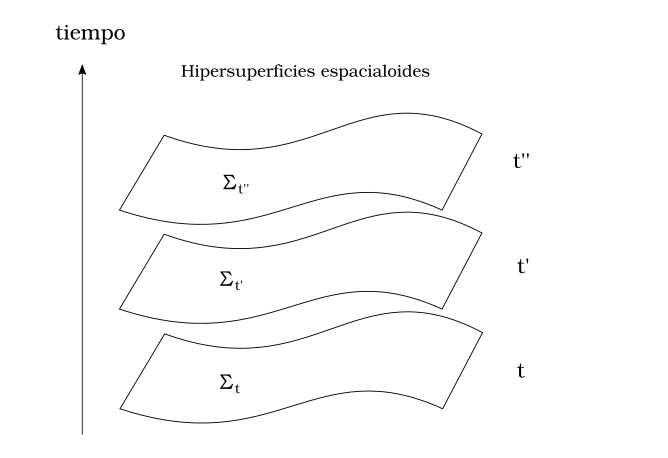
\includegraphics[width=0.7\textwidth]{Foliation.png}
\caption{Foliaci\'{o}n del espacio-tiempo en hipersuperficies espacialoides.}\label{fig:Foliation}
\end{figure}

En cada hipersuperficie $\Sigma_{t}$ se usar\'{a}n las coordenadas $y^{a}$, que se relacionar\'{a}n mediante una congruencia de curvas $\gamma$ parametrizadas por la funci\'{o}n de tiempo $t$ y vector tangente (tipo tiempo) $t^{\alpha} = d x^{\alpha} / d t$ a la curva. Estas curvas intersectan a las hipersuperficies $\Sigma_{t}$, pero no necesariamente de manera ortogonal ni tampoco se debe asumir que son geod\'{e}sicas. 

Una curva en particular $\gamma_{q}$ de la congruencia, define un mapeo de un punto $q$ en $\Sigma_{t}$ a un punto $q'$ en $\Sigma_{t'}$, y tambi\'{e}n a un punto $q''$ en $\Sigma_{t''}$, y as\'{i} sucesivamente (figura \ref{fig:curvagamma}). Para fijar las coordenadas de $q'$ y $q''$, dadas las coordenadas $y^{a}(q)$ en $\Sigma_{t}$, simplemente se impone que $y^{a}(q) = y^{a}(q') = y^{a}(q'')$. De esta manera, $y^{a}$ se mantiene constante sobre cada una de las curvas $\gamma$.

\begin{figure}[H]
\centering
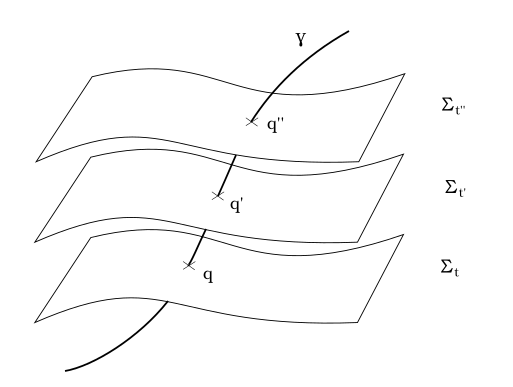
\includegraphics[width=0.5\textwidth]{Gammaintersectingqpoints.png}
\caption{Curva $\gamma$ relacionando puntos de distintas hipersuperficies.}\label{fig:curvagamma}
\end{figure}

N\'{o}tese que por construcci\'{o}n se defini\'{o} un sistema coordenado $(t, y^{a})$ en $\Omega$. As\'{i} que existe una transformaci\'{o}n entre \'{e}ste y el sistema coordenado $x^{\alpha}$, lo que permite expresar las coordenadas originales en t\'{e}rminos de las nuevas, esto es: $x^{\alpha} = x^{\alpha} (t, y^{\alpha})$. Entonces,
%
\begin{align}
\label{eq:dxalpha}
dx^{\alpha} & = \left( \frac{\partial x^{\alpha}}{\partial t} \right)_{y^{a}} dt + \left( \frac{\partial x^{\alpha}}{\partial y^{a}} \right)_{t} dy^{a} \nonumber \\
& = t^{\alpha} dt + e^{\alpha}_{a} dy^{a},
\end{align}
%
donde $t^{\alpha}=\partial x^{\alpha}/\partial t$ es el vector tangente a $\gamma$ y $e^{\alpha}_{a}=\partial x^{\alpha}/\partial y^{a}$ son los vectores tangentes a $\Sigma_{t}$.

El vector tangente $t^{\alpha}$ a la curva $\gamma$ en general no es ortogonal a $\Sigma_{t}$ (i.e., no es paralelo al vector normal $n^{\alpha}$). Ahora bien, el normal unitario es $n_{\alpha} = -N \partial_{\alpha} t$, donde $N$ es conocida como la \emph{funci\'{o}n de lapso} que se encarga de normalizar, as\'{i} que $N$ es la proyecci\'{o}n de $t^{\alpha}$ sobre el normal unitario\footnotemark. Tambi\'{e}n n\'{o}tese que $t^{\alpha}$ va a tener una proyecci\'{o}n sobre los vectores tangentes $e^{\alpha}_{a}$, estas proyecciones forman un vector tipo espacio $N^{a}$ tangente a $\Sigma_{t}$ y conocido como \emph{vector de corrimiento}.
\footnotetext{Ya que $t^{\alpha} \partial_{\alpha} t = 1$.}

\begin{center}
\begin{tikzpicture}
%
\draw (-3.5, 0) to[out=40,in=-150] 
  coordinate[pos=0.25] (aux1)(3.5, 0.5);
%
\draw[fill] (aux1) circle (1pt);
\node[label=below:$q$] at (aux1) {};
%
\coordinate (aux2) at (-2.1,2.3); 
\coordinate (aux3) at (0.9,0.7);
%\draw (aux1) ->  node [left] {$N n^{\alpha}$} (aux2);
%\draw (aux1) ->  node [above] {$N^{a} e^{\alpha}_{a}$} (aux3);
\path[->,>=stealth] (aux1) edge node [left] {$N n^{\alpha}$} (aux2);
\path[->,>=stealth] (aux1) edge node [above right] {$N^{a} e^{\alpha}_{a}$} (aux3);
%
\coordinate (aux4) at (0.4,2);
%\draw (aux1) ->  node [above] {$t^{\alpha}$} (aux4);
\path[->,>=stealth] (aux1) edge node [above] {$t^{\alpha}$} (aux4);
%
\node at (3.9, 0.5) {$\Sigma_{t}$};
\node at (-2.1, 2.7) {``l\'{i}nea'' normal};
\node at (1.5,2.4) {``l\'{i}nea'' coordenada};
%
\end{tikzpicture}
\end{center}

As\'{i}, el vector $t^{\alpha}$ se descompone como,
%
\begin{equation}
\label{eq:descompt}
t^{\alpha} = N n^{\alpha} + N^{a} e^{\alpha}_{a}.
\end{equation}

Sustituyendo \eqref{eq:descompt} en \eqref{eq:dxalpha} y tomando en cuenta que el elemento de l\'{i}nea est\'{a} dado por $ds^{2} = g_{\mu \nu} d x^{\mu} d x^{\nu}$, se sigue que en el nuevo sistema coordenado
%
\begin{equation}
\label{eq:dslapseandshift}
ds^{2} = (-N^{2} + N_{a} N^{a}) dt^{2} + 2 N_{a} dt dy^{a} + h_{ab} dy^{a} dy^{b}.
\end{equation}

%La ecuaci\'{o}n \eqref{eq:dslapseandshift} es la descomposici\'{o}n (3+1) de la m\'{e}trica. Expl\'{i}citamente se tiene
%
%\begin{equation}
%\label{eq:metric31}
%g_{AB} =
 %\begin{pmatrix}
 %-N^{2} + N_{a} N^{a} & N_{a} \\
 %N_{b} & h_{ab}
 %\end{pmatrix},
%\end{equation}
%
%\begin{equation}
%\label{eq:invmetric31}
%g^{AB} =
%\begin{pmatrix}
 %-1 / N^{2} & N^{a} / N^{2} \\
 %N^{b} / N^{2} & h^{ab} - N^{a} N^{b} / N^{2}
 %\end{pmatrix}.
%\end{equation}

Vale la pena recordar que $h_{ab}$ es la m\'{e}trica en $\Sigma_{t}$

Se puede mostrar que
%
\begin{equation}
\label{eq:elemntvol31}
\sqrt{-g} = N \sqrt{h}.
\end{equation}

Las ecuaciones \eqref{eq:descompt}, \eqref{eq:dslapseandshift} y \eqref{eq:elemntvol31} son los resultados fundamentales de la descomposici\'{o}n (3+1).

%-------------------------------------------------------------
% FOLIACI�N DE LA FRONTERA
%-------------------------------------------------------------

\subsection{Foliaci�n de la frontera}
\label{subsec:foliacionfrontera}

Consid�rese una regi�n $\Omega$ del espacio-tiempo foleada por hipersuperficies espacialoides $\Sigma_{t}$ cuya frontera son superficies (bidimensionales) cerradas $S_{t}$. $\partial \Omega$ es la uni�n de las hipersuperficies $\Sigma_{t_{1}}$, $\Sigma_{t_{2}}$ y $\mathcal{B}$ (la uni�n de todas las superficies $S_{t}$).

\begin{figure}[H]
\label{fig:OmegaandboundOmega}
\centering
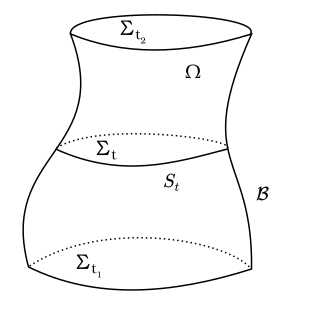
\includegraphics[width=0.3\textwidth]{Omega.png}
\caption{Regi�n $\Omega$, frontera $\partial \Omega$ y la foliaci�n.}
\end{figure}

Las superficies cerradas $S_{t}$ est�n descrita por las relaciones param�tricas $y^{a} (\theta^{w})$, donde $\theta^{w}$ son las coordenas en $S_{t}$. Se denota a $r_{a}$ como el vector normal a $S_{t}$ y se define un 4-vector asociado $r^{\alpha} = r^{a} e^{\alpha}_{a}$, que es ortogonal a $n_{\alpha}$ y satisface $r^{\alpha} r_{\alpha} = 1$.

Los vectores $e^{a}_{w} = \partial y^{a} / \partial \theta^{w}$ tangentes a $S_{t}$ expresados como 4-vectores se ven de la siguiente manera,
%
\begin{equation}
\label{eq:ealphaw}
e^{\alpha}_{w} = e^{\alpha}_{a} e^{a}_{w} = \frac{\partial x^{\alpha}}{\partial \theta^{w}}.
\end{equation}

La ecuaci�n \eqref{eq:ealphaw} ayuda a ver que las componentes de la m�trica $\sigma_{vw}$ inducida en $S_{t}$ est�n dadas por
%
\begin{equation}
\label{eq:metricSt}
\sigma_{vw} = h_{ab} e^{a}_{v} e^{b}_{w}
= (g_{\alpha \beta} e^{\alpha}_{a} e^{\beta}_{b}) e^{a}_{v} e^{b}_{w}
= g_{\alpha \beta} e^{\alpha}_{v} e^{\beta}_{w}.
\end{equation}
%
Y su inversa es denotada por $\sigma^{vw}$. Las relaciones de completez son $h^{ab} = r^{a} r^{b} + \sigma^{vw} e^{a}_{v} e^{b}_{w}$ y $g^{\alpha \beta} = -n^{\alpha} n^{\beta} + h^{ab} e^{\alpha}_{a} e^{\beta}_{b}$. Est� �ltima puede reescribirse como
%
\begin{equation}
\label{eq:complt}
g^{\alpha \beta} = -n^{\alpha} n^{\beta} + r^{\alpha} r^{\beta} + \sigma^{vw} e^{\alpha}_{v} e^{\beta}_{w}.
\end{equation}

La curvatura extr�nseca de $S_{t}$ encajada en $\Sigma_t$ est� definida por
%
\begin{equation}
\label{eq:extrinseccurvSt}
k_{vw} = e^{\alpha}_{v} e^{\beta}_{w} k_{\alpha \beta} = e^{\alpha}_{v} e^{\beta}_{w} \nabla_{\beta} r_{\alpha}.
\end{equation}
%
La traza de $k_{vw}$ no es m�s que $k = \sigma^{vw} k_{vw}$.

De manera similar a lo hecho en la secci�n \ref{subsec:3+1}, para relacionar las coordenadas $\theta^{w}$ de una superficie $S_{t}$ con las de otra superficie $S_{t}'$, se considera una congruencia de curvas $\beta$ en $\mathcal{B}$ que intersecten las superficies $S_{t}$ ortogonalmente, es decir, que vayan a lo largo de $n^{\alpha}$. Despu�s se pide que si la curva $\beta_{q}$ intersecta $S_{t}$ en $q$ con coordenada $\theta^{w}$, entonces la misma coordenada se asignada en la intersecci�n de $\beta_{q}$ con $S_{t'}$ y as� sucesivamente.

La hipersuperficie $\mathcal{B}$ est� foleada por las superficies $S_{t}$. En principio, se puede ajustar a $\mathcal{B}$ un sistema coordenado arbitrario, sin embargo conviene escoger: $z^{f} = (t, \theta^{w})$. En �stas coordenadas $dx^{\alpha} = N n^{\alpha} dt + e^{\alpha}_{w} d \theta^{w}$, as� para desplazamientos dentro de $\mathcal{B}$ el elemento de l�nea es
%
\begin{align}
\label{eq:dsB}
ds_{\mathcal{B}} & = g_{\alpha \beta} (N n^{\alpha} dt + e^{\alpha}_{v} d \theta^{v}) (N n^{\beta} dt + e^{\beta}_{w} d \theta^{w}) \nonumber \\
& = - N^{2} dt^{2} + \sigma_{vw} d \theta^{v} d \theta^{w}.
\end{align}
%
Por otro lado, la m�trica inducida $\gamma_{fg}$ en $\mathcal{B}$ tiene componentes
%
\begin{equation}
\label{eq:indmetricB}
\gamma_{fg} = g_{\alpha \beta} \left( \frac{\partial x^{\alpha}}{\partial z^{f}} \right) \left( \frac{\partial x^{\beta}}{\partial z^{g}} \right) = g_{\alpha \beta} e^{\alpha}_{f} e^{\beta}_{g}
\end{equation}
%
y la inversa se denota por $\gamma^{fg}$. La relaci�n de completes toma la forma\footnote{Como $r^{\alpha}$ es ortogonal a $S_{t}$, tambi�n lo es a $\mathcal{B}$.}
%
\begin{equation}
\label{eq:Bcompltrelation}
g^{\alpha \beta} = r^{\alpha} r^{\beta} + \gamma^{fg} e^{\alpha}_{f} e^{\beta}_{g}.
\end{equation}

Ahora, de \eqref{eq:dsB} se sigue que
%
\begin{equation}
\gamma_{fg} dz^{f} dz^{g} =  - N^{2} dt^{2} + \sigma_{vw} d \theta^{v} d \theta^{w},
\end{equation}
%
por lo que implica $\sqrt{-\gamma} = N \sqrt{\sigma}$.

Por �ltimo,  la curvatura extr�nseca $\mathcal{K}_{fg}$ de $\mathcal{B}$ dentro del espacio-tiempo est� dada por
%
\begin{equation}
\mathcal{K}_{fg} = e^{\alpha}_{f} e^{\beta}_{g} \nabla_\beta r^{\alpha},
\end{equation}
%
y su traza por $\mathcal{K} = \gamma^{fg} \mathcal{K}_{fg}$.
%---------------------------------------------------------------------------
% ACCI�N GRAVITACIONAL EN EL FORMALISMO 3+1
%---------------------------------------------------------------------------

\subsection{Acci�n gravitacional en el formalismo (3+1)}

Para construir el Hamiltoniano gravitacional se realizar� la descomposici�n (3+1) del funcional de acci�n gravitacional $S_{G}$. Por ahora s�lo se considerar�n los t�rminos $I_{EH}$ e $I_{B}$, m�s adelante se reincorporar� $I_{0}$.
%
\begin{equation}
\label{eq:SGIEHIB}
S_{G} = \frac{1}{16 \pi} \left( \int_{\Omega} R \sqrt{-g} \, d^{4} x + 2 \oint_{\partial \Omega} \varepsilon K \sqrt{|h|} \, d^{3} y \right).
\end{equation}

Como en la secci�n (\ref{subsec:foliacionfrontera}), $\Omega$ tiene por frontera a $\partial \Omega$ que es la uni�n de dos hipersuperficies espacialoides $\Sigma_{t_{1}}$ y $\Sigma_{t_{2}}$, y la hipersuperficie tipo tiempo $\mathcal{B}$ (figura \ref{fig:OmegaandboundOmega}), esto es,
%
\begin{equation}
\label{eq:domegaU}
\partial \Omega  = -\Sigma_{t_{1}} \cup \Sigma_{t_{2}} \cup \mathcal{B}.
\end{equation}
%
Con lo que el t�rmino de frontera toma la forma,
%
\begin{equation}
\label{eq:IB31}
2 \oint_{\partial \Omega} \varepsilon K \sqrt{|h|} \, d^{3} y = 2 \int_{\Sigma_{t_1}} K \sqrt{|h|} \, d^{3} y - 2 \int_{\Sigma_{t_2}} K \sqrt{|h|} \, d^{3} y + 2 \int_{\mathcal{B}} \mathcal{K} \sqrt{-\gamma} \, d^{3} z.
\end{equation}

La regi�n $\Omega$ es foleada por las hipersuperficies espacialoides $\Sigma_{t}$, sobre las cuales el escalar de Ricci est� dado por
%
\begin{equation}
\label{eq:Riccionsigma}
R = ^{(3)}R + K^{ab} K_{ab} - K^{2} - 2 \nabla_{\alpha} (n^{\beta} \nabla_{\beta} n^{\alpha} - n^{\alpha} \nabla_{\beta} n^{\beta}),
\end{equation}
%
donde $^{(3)}R$ es el escalar de Ricci construido a partir de $h_{ab}$. De esta forma, el t�rmino de Einstein-Hilbert queda reescrito como
%
\begin{equation}
\int_{\Omega} R \sqrt{-g} \, d^{4} x = \int^{t_{1}}_{t_{2}} dt \left[ \int_{\Sigma_{t}} (^{(3)}R + K^{ab} K_{ab} - K^{2}) N \sqrt{h} \, d^{3} y - 2 \oint_{\partial \Omega} (n^{\beta} \nabla_{\beta} n^{\alpha} - n^{\alpha} \nabla_{\beta} n^{\beta}) \, d \Sigma_{\alpha} \right],
\end{equation}
%
donde se us� la expresi�n \eqref{eq:elemntvol31}, \eqref{eq:Riccionsigma} y el teorema de Gauss. Como la frontera es la uni�n de varias hipersuperficies, ecuaci�n \eqref{eq:domegaU}, la integral sobre $\partial \Omega$ se descompone en integrales sobre $\Sigma_{t_{1}}$, $\Sigma_{t_{2}}$ y $\mathcal{B}$. El trato de la integral sobre $\Sigma_{t_{1}}$ y $\Sigma_{t_{2}}$ es el mismo (salvo por un signo global), as� que solamente es necesario mostrar uno de estos c�lculos,
%
\begin{align}
-2 \int_{\Sigma_{t_{1}}} (n^{\beta} \nabla_{\beta} n^{\alpha} - n^{\alpha} \nabla_{\beta} n^{\beta}) \, d \Sigma_{\alpha} & = -2 \int_{\Sigma_{t_{1}}} (\nabla_{\beta} n^{\beta}) \sqrt{h} \, d^{3} y \nonumber \\
& = -2 \int_{\Sigma_{t_{1}}} K \sqrt{h} \, d^{3} y.
\end{align}
%
La integral sobre $\Sigma_{t_{2}}$ da el mismo resultado pero con signo contrario. Ambos resultados se cancelan con las integrales sobre $\Sigma_{t_{1}}$ y $\Sigma_{t_{2}}$ de \eqref{eq:IB31}. Por otro lado, la integral sobre $\mathcal{B}$ contribuye con
%
\begin{align}
-2 \int_{\mathcal{B}} (n^{\beta} \nabla_{\beta} n^{\alpha} - n^{\alpha} \nabla_{\beta} n^{\beta}) \, d \Sigma_{\alpha} & = -2 \int_{\mathcal{B}} (n^{\beta} \nabla_{\beta} n^{\alpha}) r_{\alpha} \sqrt{-\gamma} \, d^{3} z \nonumber \\
& = 2 \int_{\mathcal{B}} n^{\alpha} n^{\beta} \nabla_{\beta} r_{\alpha} \sqrt{-\gamma} \, d^{3} z.
\end{align}

Juntando los resultados, el funcional de acci�n gravitacional (a�n sin el t�rmino $I_{0}$) queda de la siguiente manera
%
\begin{equation}
\label{eq:SGIEHIB}
S_{G} = \frac{1}{16 \pi} \int^{t_{2}}_{t_{1}} dt \left[ \int_{\Sigma_{t}} (^{(3)}R + K^{ab} K_{ab} - K^{2}) N \sqrt{h} \, d^{3} y + 2 \int_{\mathcal{B}} (\mathcal{K} + n^{\alpha} n^{\beta} \nabla_{\beta} r_{\alpha}) \sqrt{-\gamma} \, d^{3} z\right].
\end{equation}

Ahora bien, a partir de las relaciones de completez \eqref{eq:Bcompltrelation} y \eqref{eq:complt} se manipula $(\mathcal{K} + n^{\alpha} n^{\beta} \nabla_{\beta} r_{\alpha})$. Primero,
%
\begin{equation}
\mathcal{K} = \gamma^{fg} \mathcal{K}_{fg} = \gamma^{fg} (e^{\alpha}_{f} e^{\beta}_{g} \nabla_{\beta} r_{\alpha}) = (g^{\alpha \beta} - r^{\alpha} r^{\beta}) \nabla_{\beta} r_{\alpha},
\end{equation}
%
que al sumar $n^{\alpha} n^{\beta} \nabla_{\beta} r_{\alpha}$, se obtiene
%
\begin{equation}
\label{eq:manipulationk}
(g^{\alpha \beta} - r^{\alpha} r^{\beta}) \nabla_{\beta} r_{\alpha} + n^{\alpha} n^{\beta} \nabla_{\beta} r_{\alpha} = \sigma^{vw} e^{\alpha}_{v} e^{\beta}_{w} (\nabla_{\beta} r_{\alpha}) = \sigma^{vw} k_{vw} = k.
\end{equation}

Sustituyendo (\ref{eq:manipulationk}) en (\ref{eq:SGIEHIB}) y adem�s, tomando en cuenta que $\mathcal{B}$ est� foleada por las superficies cerradas $S_{t}$ (as� que $\sqrt{-\gamma} d^{3} z = N \sqrt{\sigma} dt d^{2} \theta$), entonces,
%
\begin{equation}
\label{eq:LagSg}
S_{G} = \frac{1}{16 \pi} \int^{t_{2}}_{t_{1}} dt \left[ \int_{\Sigma_{t}} (^{(3)}R + K^{ab} K_{ab} - K^{2}) N \sqrt{h} \, d^{3} y + 2 \oint_{S_{t}} (k - k_{0}) N \sqrt{\sigma} \, d^{2} \theta \right].
\end{equation}

N�tese que ahora s� se incluy� $I_{0}$ al escribir el t�rmino $k_{0}$ en la integral sobre $S_{t}$. La elecci�n de $k_{0}$ como la curvatura extr�nseca de $S_{t}$ encajada en el espacio plano previene que la integral diverja en el l�mite $S_{t} \rightarrow \infty$, asegurando que $S_{G}$ est� bien definido para cualquier espacio-tiempo asint�ticamente plano.
%---------------------------------------------------------------------------
% HAMILTONIANO GRAVITACIONAL
%---------------------------------------------------------------------------

\subsection{Hamiltoniano Gravitacional}

En el formalismo (3+1) el sistema es descrito por $h_{ab}$y por c�mo �sta cambia a lo largo del \emph{flujo de tiempo}, es decir, del campo vectorial $t^{\alpha} = N n^{\alpha} + N^{\alpha}$. Las variables fundamentales son pues, la m�trica $h_{ab}$ y su \emph{momento can�nicamente conjugado} $p^{ab}$,
%
\begin{equation}
p^{ab} = \frac{\partial \mathcal{L}_{G}}{\partial \dot{h}_{ab}}.
\end{equation}
%
Aqu�, $16 \pi \mathcal{L}_{G} = (^{(3)}R + K^{ab} K_{ab} - K^{2}) N \sqrt{h}$, y $\dot{h}_{ab}$ es el cambio de la m�trica a trav�s del flujo de tiempo, esto es,
%
\begin{equation}
\dot{h}_{ab} = \pounds_{t} h_{ab}.
\end{equation}

Recordando que $h_{ab} = g_{\alpha \beta} e^{\alpha}_{a} e^{\beta}_{b}$, se calcula la derivada de Lie de la m�trica $g_{\mu \nu}$ a lo largo del campo vectorial $t$, despu�s se proyecta en la hipersuperficie $\Sigma_{t}$ y se obtiene que
%
\begin{equation}
\label{eq:doth}
\dot{h}_{ab} = 2 N K_{ab} + D_{b} N_{a} + D_{a} N_{b},
\end{equation}
%
donde $D_{a}$ es la derivada covariente en $\Sigma_{t}$ combatible con $h_{ab}$.
%\begin{equation}
%\dot{h}_{ab} = \pounds_{t} (g_{\alpha \beta} e^{\alpha}_{a} e^{\beta}_{b}) = (\pounds_{t} g_{\alpha %\beta}) e^{\alpha}_{a} e^{\beta}_{b},
%\end{equation}
%
%\begin{align}
%\pounds_{t} g_{\alpha \beta} & = \nabla_{\beta} t_{\alpha} + \nabla_{\alpha} t_{\beta} \nonumber \\
%& = \nabla_{\beta} (N n_{\alpha} + N_{\alpha}) + \nabla_{\alpha} (N n_{\beta} + N_{\beta}) \nonumber \\
%& = n_{\alpha} \partial_{\beta} N + n_{\beta} \partial_{\alpha} N + N (\nabla_{\beta} n_{\alpha} + \nabla_{\alpha} n_{\beta}) + \nabla_{\beta} N_{\alpha} + \nabla_{\alpha} N_{\beta}.
%\end{align}
%
Luego se despeja la curvatura extr�nseca de \eqref{eq:doth}, para poder ver la dependencia en $\dot{h}_{ab}$ del funcional de acci�n gravitacional, entonces,
%
\begin{equation}
\label{eq:Kab(doth)}
K_{ab} = \frac{1}{2 N} \left( \dot{h}_{ab} - D_{b} N_{a} - D_{a} N_{b} \right).
\end{equation}

De la ecuaci�n anterior, \eqref{eq:Kab(doth)}, n�tese que solamente la parte de volumen de la densidad Lagrangiana de gravedad depende de $\dot{h}_{ab}$ (ver \eqref{eq:LagSg}), as� que para facilitar las cosas, se analizar� s�lo esa parte, entonces
%
\begin{align}
\label{eq:pabADM}
(16 \pi) p^{ab} & = \frac{\partial K_{mn}}{\partial \dot{h}_{ab}} \frac{\partial}{\partial K_{mn}} \left( 16 \pi \mathcal{L}_{G} \right) \nonumber \\
& = \frac{\partial K_{mn}}{\partial \dot{h}_{ab}} \frac{\partial}{\partial K_{mn}} \left( [^{(3)}R + (h^{ac} h^{bd} - h^{ab} h^{cd}) K_{ab} K_{cd}] N \sqrt{h} \right) \nonumber \\
& = \sqrt{h} (K^{ab} - K h^{ab}).
\end{align}

Haciendo la transformaci�n de Legendre $\mathcal{H}_{G} = p^{ab} \dot{h}_{ab} - \mathcal{L}_{G}$, la parte de volumen de la densidad Hamiltoniana es
%
\begin{align}
16 \pi \mathcal{H}_{G} & = \sqrt{h} (K^{ab} - K h^{ab}) (2 N K_{ab} + D_{b} N_{a} + D_{a} N_{b}) \nonumber \\
& \quad - (^{(3)}R + K^{ab} K_{ab} - K^{2}) N \sqrt{h} \nonumber \\
& = (K^{ab} K_{ab} - K^{2} - ^{(3)}R) N \sqrt{h} + 2 (K^{ab} - K h^{ab}) D_{b} N_{a} \sqrt{h} \nonumber \\
& = (K^{ab} K_{ab} - K^{2} - ^{(3)}R) N \sqrt{h} + 2 D_{b} [(K^{ab} - K h^{ab}) N_{a}] \sqrt{h} \nonumber \\
& \quad - 2 D_{b} (K^{ab} - K h^{ab}) N_{a} \sqrt{h}.
\end{align}

El Hamiltoniano gravitacional lo obtenemos integrando $\mathcal{H}_{G}$ sobre $\Sigma_{t}$ y sumando los t�rminos de frontera,
%
\begin{align}
\label{eq:HG}
16 \pi H_{G} & = \int_{\Sigma_{t}} 16 \pi \mathcal{H}_{G} \, d^{3} y - 2 \oint_{S_{t}} (k - k_{0}) N \sqrt{\sigma} \, d^{2} \theta \nonumber \\
& = \int_{\Sigma_{t}} \left[ N (K^{ab} K_{ab} - K^{2} - ^{(3)}R) - 2 N_{a} D_{b} (K^{ab} - K h^{ab}) \right] \sqrt{h} \, d^{3} y \nonumber \\
& \quad + 2 \oint_{S_{t}} (K^{ab} - K h^{ab}) N_{a} d S_{b} - 2 \oint_{S_{t}} (k - k_{0}) N \sqrt{\sigma} d^{2} \theta \nonumber \\
& = \int_{\Sigma_{t}} \left[ N (K^{ab} K_{ab} - K^{2} - ^{(3)}R) - 2 N_{a} D_{b} (K^{ab} - K h^{ab}) \right] \sqrt{h} \, d^{3} y \nonumber \\
& \quad - 2 \oint_{S_{t}} \left[ (k - k_{0}) N - (K^{ab} - K h^{ab}) N_{a} r_{b} \right] \sqrt{\sigma} d^{2} \theta,
\end{align}
%
donde $d S_{b} = r_{b} \sqrt{\sigma} d^{2} \theta$.

En el Hamiltoniano, ecuaci�n \eqref{eq:HG}, $K^{ab}$ representa a las funciones $h^{ab}$ y $p^{ab}$, expl�citamente
%
\begin{equation}
\label{eq:Kph}
\sqrt{h} K^{ab} = 16 \pi ( p^{ab} - \frac{1}{2} p h^{ab}).
\end{equation}
%
con $p:= h_{ab} p^{ab}$.
%---------------------------------------------------------------------------
% ECUACIONES DE CAMPO EN FORMA HAMILTONIANA
%---------------------------------------------------------------------------

\subsection{Ecuaciones del campo gravitacional}

Para obtener las ecuaciones de campo gravitacional en forma Hamiltoniana se hace la variaci\'{o}n de la acci\'{o}n\footnotemark $S = S_{G}$, con $S_{G}$ escrita en forma can\'{o}nica
\footnotetext{Por el momento estamos considerando que estamos en vac\'{i}o, i.e. $S_{M} = 0$.}
%
\begin{equation}
S_{G} = \int^{t_2}_{t_1} dt \left[ \int_{\Sigma_{t}} p^{ab} \dot{h}_{ab} \, d^{3} y - H_{G} \right],
\end{equation}
%
respecto a las variables independientes $N$, $N^{a}$, $h_{ab}$, y $p^{ab}$, sujetas a las condiciones
%
\begin{equation}
\label{eq:boundcondh}
\delta N \Big|_{S_{t}} = \delta N^{a} \Big|_{S_{t}} = \delta h_{ab} \Big|_{S_{t}} = 0,
\end{equation}
%
y sin condici\'{o}n sobre $\delta p^{ab}$ de anularse en la frontera $S_{t}$. La variaci\'{o}n da
%
\begin{equation}
\label{eq:varSG31}
\delta S_{G} = \int^{t_1}_{t_2} dt \left[ \int_{\Sigma_{t}} (p^{ab} \delta \dot{h}_{ab} + \dot{h}_{ab} \delta p^{ab}) \, d^{3} y - \delta H_{G} \right].
\end{equation}

Comenzaremos calculando la variaci\'{o}n del Hamiltoniano gravitacional $H_{G}$. Iniciamos con la variaci\'{o}n con respecto a las funciones no din\'{a}micas, $N$ y $N^{a}$:
%
\begin{equation}
\label{eq:varHcrNNa}
16 \pi \delta_{N} H_{G} = \int_{\Sigma_{t}} (- \hat{\mathcal{C}} \delta N - 2 \hat{\mathcal{C}}_{a} \delta N^{a}) \, d^{3} y,
\end{equation}
%
(por la condici\'{o}n \eqref{eq:boundcondh} impuesta en $\delta N \Big|_{S_{t}}$ y $\delta N^{a} \Big|_{S_{t}}$ el t\'{e}rmino de frontera se anula) con
%
\begin{equation}
\hat{\mathcal{C}} := (^{(3)}R + K^{2} - K^{ab} K_{ab}) \sqrt{h}, \qquad \hat{\mathcal{C}}_{a} := [D_{b} (K_{a}^{b} - K \delta_{a}^{b})] \sqrt{h}.
\end{equation}

Para hacer la variaci\'{o}n de $H_{G}$ respecto a $p^{ab}$ y $h_{ab}$ hay que expresar el Hamiltoniano en t\'{e}rminos de $p^{ab}$ y $h_{ab}$, para ello se usa \eqref{eq:Kph} en \eqref{eq:HG}, de este modo,
%
\begin{align}
\label{eq:16piHG}
16 \pi H_{G} & = \int_{\Sigma_{t}} \left[ N h^{-1/2} (\hat{p}_{ab} \hat{p}^{ab} - \frac{1}{2} \hat{p}^{2}) - N h^{1/2} \, ^{(3)}R - 2 N_{a} h^{1/2} D_{b} (h^{-1/2} \hat{p}^{ab}) \right] \, d^{3} y
\nonumber \\
& \quad - 2 \oint_{S_{t}} \left[ N (k - k_{0}) - N_{a} h^{-1/2} \hat{p}^{ab} r_{b} \right] \sqrt{\sigma} \, d^{2} \theta.
\end{align}
%
Aqu\'{i} se defini\'{o} $\hat{p}^{ab} = 16 \pi p^{ab}$ ($\hat{p}_{ab} = 16 \pi p_{ab}$). Haciendo la variaci\'{o}n con respecto a $\hat{p}^{ab}$, se tiene
%
\begin{align}
\label{eq:varHcrp}
(16 \pi) \delta_{p} H_{G} & = \int_{\Sigma_{t}} N h^{-1/2} \delta_{p}(\hat{p}_{ab} \hat{p}^{ab} - \frac{1}{2} \hat{p}^{2}) \, d^{3} y - 2 \delta_{p} \int_{\Sigma_{t}} N_{a} h^{1/2} D_{b} (h^{-1/2} \hat{p}^{ab}) \, d^{3} y \nonumber \\
& \quad + 2 \oint_{S_{t}} N_{a} h^{-1/2} \delta \hat{p}^{ab} r_{b} \sqrt{\sigma} \, d^{2} \theta \nonumber \\
& = \int_{\Sigma_{t}} 2 \left[ N h^{-1/2} (\hat{p}_{ab} - \frac{1}{2} \hat{p} h_{ab}) + D_{(b} N_{a)} \right] \delta \hat{p}^{ab} \, d^{3} y \nonumber \\
& = \int_{\Sigma_{t}} \mathcal{H}_{ab} \delta \hat{p}^{ab} \, d^{3} y.
\end{align}

Ahora, se hace la variaci\'{o}n de $H_{G}$ con respecto a $h_{ab}$. Lo haremos por partes, primero el t\'{e}rmino de volumen\footnotemark
\footnotetext{La integral sobre $S_{t}$ viene de aplicar el teorema de Gauss al t\'{e}rmino $2 N_{a} h^{1/2} D_{b} (h^{-1/2} \hat{p}^{ab})$ en la ecuaci\'{o}n \eqref{eq:16piHG}.}
%
\begin{align}
(16 \pi) \delta_{h} H_{\Sigma} & = \int_{\Sigma_{t}} \left[ -N h^{-1} (\hat{p}^{ab} \hat{p}_{ab} - \frac{1}{2} \hat{p}^{2}) \delta_{h} h^{1/2} + N h^{-1/2} \delta_{h} (\hat{p}^{ab} \hat{p}_{ab} - \frac{1}{2} \hat{p}^{2}) \right. \nonumber \\
& \quad \left. - N \delta_{h} (h^{1/2} \, ^{(3)}R) + 2 \delta_{h} (\hat{p}^{ab} D_{b} N_{a}) \right] \, d^{3} y - 2 \delta_{h} \oint_{S_{t}} N_{a} h^{-1/2} \hat{p}^{ab} r_{b} \sqrt{\sigma} \, d^{2} \theta.
\end{align}
%
Por la condici\'{o}n de frontera \eqref{eq:boundcondh}, la variaci\'{o}n de la integral sobre $S_{t}$ se anula. Usando $^{(3)}R = R_{ab} h^{ab}$ y las relaciones $\delta h^{ab} = -h^{ac} h^{db} \delta h_{cd}$ y $\delta_{h} h^{1/2} = \frac{1}{2} h^{1/2} h^{ab} \delta h_{ab}$, es posible mostrar que
%
\begin{align*}
\delta_{h} (h^{1/2} \, ^{(3)}R) & = - h^{1/2} (R^{ab} - \frac{1}{2}\, ^{(3)}R h^{ab}) \delta h_{ab} + h^{1/2} D_{c} (h^{ab} \delta \Gamma^{c}\,_{ab} - h^{ac} \delta \Gamma^{b}\,_{ab}) \\
& = - h^{1/2} G^{ab} \delta h_{ab} + h^{1/2} D_{c} v^{c}.
\end{align*}
%
El resto de las variaciones son:
%
\begin{equation*}
\delta_{h} (\hat{p}^{ab} \hat{p}_{ab} - \frac{1}{2} \hat{p}^{2}) = 2(\hat{p}^{a}_{c} \hat{p}^{cb} - \frac{1}{2} \hat{p} \hat{p}^{ab}) \delta h_{ab},
\end{equation*}
%
\begin{equation*}
\delta_{h} D_{b} N_{a} = (D_{b} N^{c}) \delta h_{ac} + h_{ac} N^{d} \delta \Gamma^{c}\,_{bd}.
\end{equation*}
%
Con esto se sigue que
%
\begin{align}
\label{eq:vc}
(16 \pi) \delta_{h} H_{\Sigma} & = \int_{\Sigma_{t}} \left[-\frac{1}{2} N h^{-1/2} (\hat{p}^{cd} \hat{p}_{cd} - \frac{1}{2} \hat{p}^{2}) h^{ab} + 2 N h^{-1/2} (\hat{p}^{a}_{c} \hat{p}^{bc} - \frac{1}{2} \hat{p} \hat{p}^{ab}) \right. \nonumber \\
& \quad \left. + N h^{1/2} G^{ab} + 2 \hat{p}^{c (a} D_{c} N^{b)} \right] \delta h_{ab} \, d^{3} y \nonumber \\
& \quad + \int_{\Sigma_{t}} \left(-N h^{1/2} D_{c} v^{c} + 2 \hat{p}^{b}_{c} N^{d} \delta \Gamma^{c}\,_{bd} \right) \, d^{3} y.
\end{align}

Ahora bien, conviene analizar la segunda integral por separado. Primero,
%
\begin{align*}
- \int_{\Sigma_{t}} N h^{1/2} D_{c} v^{c} \, d^{3} y & = \int_{\Sigma_{t}} (\partial_{c} N) v^{c} h^{1/2} \, d^{3} y - \oint_{S_{t}} N v^{c} r_{c} \sqrt{\sigma} \, d^{2} \theta \\
& = \int_{\Sigma_{t}} (\partial_{c} N) v^{c} h^{1/2} \, d^{3} y + \oint_{S_{t}} N h^{ab} \delta (\partial_{c} h_{ab}) r^{c} \sqrt{\sigma} d^{2} \theta \\
& = - \int_{\Sigma_{t}} (h^{ab} \partial^{d} N - h^{bd} \partial^{a} N) (D_{d} \delta h_{ab}) h^{1/2} \, d^{3} y \\
& \quad + \oint_{S_{t}} N h^{ab} (\partial_{c} \delta h_{ab}) r^{c} \sqrt{\sigma} d^{2} \theta \\
& = \int_{\Sigma_{t}} (h^{ab} D_{d} D^{d} - D^{b} D^{a} N) \delta h_{ab} h^{1/2} \, d^{3} y \\
& \quad + \oint_{S_{t}} N h^{ab} (\partial_{c} \delta h_{ab}) r^{c} \sqrt{\sigma} d^{2}.
\end{align*}
%
Donde se us\'{o} la versi\'{o}n tridimensional de la ecuaci\'{o}n \eqref{eq:vnh} y la siguiente relaci\'{o}n:
%
\begin{equation}
\label{eq:varGamma3D}
\delta \Gamma^{c}_{ab} = \frac{1}{2} h^{cd} \left[D_{b} (\delta h_{da}) + D_{a} (\delta h_{db}) - D_{d} (\delta h_{ab}) \right],
\end{equation}
%
para tener: $v^{c} = 1/2 (h^{ab} h^{cd} - h^{ac} h^{bd}) [D_{b} (\delta h_{da}) + D_{a} (\delta h_{db}) - D_{d} (\delta h_{ab})]$, y al contraer con $\partial_{c} N$ (aprovechando la antisimetr\'{i}a en $a$ y $d$) obtener el resultado. Para el otro t\'{e}rmino de la segunda integral, tenemos que
%
\begin{align*}
\int_{\Sigma_{t}} 2 \hat{p}^{b}_{c} N^{d} \delta \Gamma^{c}\,_{bd} \, d^{3} y & = \int_{\Sigma_{t}} h^{1/2} \hat{p}^{ab} N^{d} D_{d} (\delta h_{ab}) h^{-1/2} \, d^{3} y \\
& = - \int_{\Sigma_{t}} D_{d} (h^{-1/2} \hat{p}^{ab} N^{d}) \delta h_{ab} h^{1/2} \, d^{3} y,
\end{align*}
%
donde tambi\'{e}n se us\'{o} \eqref{eq:varGamma3D} y depu\'{e}s, al integrar por partes, se utiliz\'{o} el teorema de Gauss y la condici\'{o}n de frontera $\delta h_{ab} \vert_{S_{t}} = 0$. As\'{i},
%
\begin{equation}
\label{eq:varHSigma}
(16 \pi) \delta_{h} H_{\Sigma} = \int_{\Sigma_{t}} \hat{\mathcal{P}}^{ab} \delta h_{ab} \, d^{3} y + \oint_{S_{t}} N h^{ab} (\partial_{c} \delta h_{ab}) r^{c} \sqrt{\sigma} d^{2}.
\end{equation}
%
Donde
%
\begin{align*}
\hat{\mathcal{P}}^{ab} & := h^{1/2} N G^{ab} - \frac{1}{2} N h^{-1/2} (\hat{p}^{cd} \hat{p}_{cd} - \frac{1}{2} \hat{p}^{2}) h^{ab} + 2 N h^{-1/2} (\hat{p}^{a}_{c} \hat{p}^{bc} - \frac{1}{2} \hat{p} \hat{p}^{ab}) \\
& \quad -h^{1/2} (D^{a} D^{b} N - h^{ab} D_{c} D^{c} N) - h^{1/2} D_{c} (h^{-1/2} \hat{p}^{ab} N^{c}) + 2 \hat{p}^{c(a} D_{c} N^{b)}.
\end{align*}

Pasando al t\'{e}rmino de frontera, al hacer la variaci\'{o}n con respecto a $h_{ab}$ se obtiene,
%
\begin{equation}
\label{eq:varHS}
(16 \pi) \delta_{h} H_{S} = -2 \oint_{S_{t}} N \delta k \sqrt{\sigma} \, d^{2} \theta = - \oint_{S_{t}} N h^{ab} (\partial_{c} \delta h_{ab}) r^{c} \sqrt{- \sigma} \, d^{2} \theta.
\end{equation}

Haciendo la suma de \eqref{eq:varHSigma} con \eqref{eq:varHS} se llega a que la variaci\'{o}n con respecto a $h_{ab}$ de $H_{G}$ es
%
\begin{equation}
\label{eq:varHcrh}
(16 \pi) \delta_{h} H_{G} = \int_{\Sigma_{t}} \hat{\mathcal{P}}^{ab} \delta h_{ab} \, d^{3} y
\end{equation}

Finalmente juntando los resultados \eqref{eq:varHcrNNa}, \eqref{eq:varHcrp} y \eqref{eq:varHcrh} se obtiene que la variaci\'{o}n del Hamiltoniano gravitacional, bajo las condiciones \eqref{eq:boundcondh}, est\'{a} dada por,
%
\begin{equation}
\label{eq:varHG}
\delta H_{G} = \int_{\Sigma_{t}} \left( \mathcal{P}^{ab} \delta h_{ab} + \mathcal{H}_{ab} \delta p^{ab} - \mathcal{C} \delta N - 2 \mathcal{C}_{a} \delta N^{a} \right) \, d^{3} y,
\end{equation}
%
con $\mathcal{P}^{ab} := \hat{\mathcal{P}}^{ab} / (16 \pi)$, $\mathcal{C} := \hat{\mathcal{C}} / (16 \pi)$ y $\mathcal{C}^{a} := \hat{\mathcal{C}}^{a} / (16 \pi)$.

Regresando a la variaci\'{o}n del funcional de acci\'{o}n gravitacional, ecuaci\'{o}n \eqref{eq:varSG31}, integrando por partes se obtiene como resultado
%
\begin{equation}
\label{varSGHamiltonianform}
\delta S_{G} = \int^{t_{2}}_{t_{1}} dt \int_{\Sigma_{t}} \left[ (\dot{h}_{ab} - \mathcal{H}_{ab}) \delta p^{ab} - (\dot{p}^{ab} + \mathcal{P}^{ab}) \delta h_{ab} + \mathcal{C} \delta N + 2 \mathcal{C}_{a} \delta N^{a} \right] \, d^{3} y.
\end{equation}
%
Imponiendo que la acci\'{o}n sea estacionaria implica
%
\begin{equation}
\label{eq:fieldequationsHamiltonianform}
\dot{h}_{ab} = \mathcal{H}_{ab}, \quad \dot{p}^{ab} = - \mathcal{P}^{ab}, \quad \mathcal{C} = 0, \quad \mathcal{C}^{a} = 0.
\end{equation}
%
Estas son las ecuaciones de Einstein (en vac\'{i}o) en la forma Hamiltoniana. Las primeras dos rigen la evoluci\'{o}n de las variables conjugadas $h_{ab}$ y $p^{ab}$; las \'{u}ltimas dos se conocen como \emph{constricciones Hamiltoniana y de difeomorfismos (o momento)} de la Relatividad General, respectivamente. Expl\'{i}citamente las constricciones son
%
\begin{equation}
\label{eq:constrictions}
\mathcal{C} = \left(^{(3)}R + K^{2} - K^{ab} K_{ab} \right) \sqrt{h} = 0, \qquad \mathcal{C}_{a} = \left[D_{b} (K^{ab} - K h^{ab}) \right] \sqrt{h} = 0.
\end{equation}
%
Entonces, en la formulaci\'{o}n Hamiltoniana para encontrar una soluci\'{o}n a las ecuaciones de Einstein se hace una foliaci\'{o}n del espacio-tiempo escogiendo la \emph{funci\'{o}n de lapso} $N$ y el \emph{vector de corrimiento} $N^{a}$, despu\'{e}s se escogen los valores iniciales para $h_{ab}$ y $K_{ab}$ de tal manera que satisfagan las constricciones (\ref{eq:constrictions}) y entonces se determina la evoluci\'{o}n de los valores iniciales usando las ecuaciones Hamiltonianas $\dot{h}_{ab} = \mathcal{H}_{ab}$ y $\dot{p}^{ab} = - \mathcal{P}^{ab}$, que equivalentemente se pueden escribir como
%
\begin{equation}
\dot{h}_{ab} = 2 N K_{ab} + \pounds_{N} h_{ab}
\end{equation}
%
y
%
\begin{equation}
\dot{K}_{ab} = D_{b} D_{a} N - N (R_{ab} + K K_{ab} - 2 K^{c}_{a} K_{bc}) + \pounds_{N} K_{ab}.
\end{equation}

\subsection{Espacio Fase}

La formulaci�n Hamiltoniana permite hacer un estudio del espacio fase de la Relatividad General. Habiendo hecho las descomposici�n 3+1, se tiene que las variables independientes son $N$, $N^{a}$ (�stas dos no din�micas) y $h_{ab}$ que respectivamente cada una tiene como momento conjugado a
%
\begin{align}
\Pi & = \frac{\partial \mathcal{L}_{G}}{\partial \dot{N}} = 0, \\
\Pi_{a} & = \frac{\partial \mathcal{L}_{G}}{\partial \dot{N}_{a}} = 0, \\
p^{ab} & = \frac{\partial \mathcal{L}_{G}}{\partial \dot{h}_{ab}} = \frac{\sqrt{h}}{16 \pi} (K^{ab} - K h^{ab}).
\end{align}
%
De esta manera, el espacio fase coordenado por $(N, N^{a}, h_{ab}, \Pi, \Pi_{a}, p^{ab})$, tiene la siguiente estructura simpl�ctica,
%
\begin{align}
\{N(t, y), \Pi(t, y')\} & = \delta(y - y'), \\
\{N^{a}(t, y), \Pi_{b}(t, y')\} & = \delta^{a}_{b} \delta(y - y'), \\
\{h_{ab}(t, y), p^{cd}(t, y')\} & = \delta^{c}_{(a} \delta^{d}_{b)} \delta(y - y'),
\end{align}
%
y el resto de los par�ntesis de Poisson son nulos.

Ahora bien, dado que $S_{G}$ contiene derivadas temporales de $h_{ab}$ por medio de los t�rminos que dependen de la curvatura extr�nseca, pero no hay derivadas temporales de $N$ ni de $N^{a}$, implica que el Lagrangiano sea singular y en consecuencia hay constricciones primarias. Las constricciones limitan la evoluci�n del sistema a una regi�n restringida del espacio fase, definen una superficie de constricci�n y adem�s las constricciones primarias generan transformaciones de norma sobre la superficie de constricci�n.

De la definici�n para los momentos conjugados se obtiene que las constricciones primarias son las siguientes,
%
\begin{align*}
\mathcal{C} & = \Pi = 0 \\
\mathcal{C}_{a} & = \Pi_{a} = 0. \\
\end{align*}
%
Es importante remarcar que $\Pi$ y $\Pi_{a}$ no son cero en todo el espacio fase, �nicamente en la superficie de constricci�n.

As�, la parte de la acci�n $S_{G}$ que va como $N \mathcal{C} + N^{a} \mathcal{C}_{a}$ es cero y la din�mica es pura norma. Por lo tanto, la descripci�n del sistema en el espacio fase tiene como variables fundamentales $h_{ab}$ y $p^{ab}$, mientras que la \emph{funci�n de lapso} y el \emph{vector de corrimiento} juegan el papel de multiplicadores de Lagrange.

%-------------------------------------------------------------
% THE NEW VARIABLESº
%-------------------------------------------------------------

\chapter{Relatividad General en Variables de Conexi\'{o}n}

Al realizar la formulaci�n Hamiltoniana a trav�s del formalismo ADM se obtienen las variables can�nicas $h_{ab}$ y $p^{ab}$ que est�n sujetas a cuatro constricciones $\mathcal{C}=0$ y $\mathcal{C}^{a}=0$ ($a=1,2,3$) \eqref{eq:constrictions}. Estas constricciones tienen una complicada dependencia no polinomial de las variables can�nicamente conjugadas, lo que ha hecho pr�cticamente imposible construir la representaci�n de momento en los intentos de cuatizaci�n con estas variables. Sin embargo, a mediados de los 80's A. Ashtekar not� que el espacio fase gravitacional podr�a reformularse en t�rminos de un nuevo par de variables can�nicas que simplifican las constricciones \cite{Ashtekar86, Ashtekar87}. Estas variables son ciertas conexiones de esp�n modificadas de aquellas construidas por A. Sen para los espinores $SL(2, \mathbb{C})$ \cite{Sen1, Sen2} y su momento can�nicamente conjugado. En esta nueva formulaci�n de la Relatividad General, en t�rminos de la conexi�n modificada y de su momento conjugado, se simplifica notablemente la forma de las constricciones y con ello la b�squeda de una teor�a cu�ntica de la Relatividad General. Adem�s, algo muy importante por destacar de esta nueva formulaci�n Hamiltoniana, es que la estructura matem�tica de la teor�a de Einstein se ve como una teor�a tipo Yang-Mills.

Aunque en esta formulaci�n las constricciones tienen una forma m�s sencilla de manejar, las variables fundamentales son complejas, lo que gener� problemas con la implementaci�n de las \emph{condiciones de realidad}. Para lidiar con esto, J. F. Barbero propuso una variante en la cual la conexi�n es real \cite{Barbero}, y es conocida como la conexi�n de Ashtekar-Barbero. La relaci�n entre las variables reales y complejas es en cierta medida clarificada por el par�metro de Barbero-Immirzi, $\beta$; las nuevas variables corresponden a las (anti-)auto-duales para $\beta = \pm i$ y a las reales para cualquier $\beta \in \mathbb{R}$ \cite{Immirzi, RovelliThiemann}.
%
%Para incorporar espinores a la teor�a se debe extender el espacio fase. Ashtekar originalmente se bas� en el c�lculo espinorial $\mathrm{SL}(2,\mathbb{C})$, pero aqu� la extensi�n del espacio fase se har� mediante el uso de triadas \cite{Vega}, pues permite ver de manera m�s clara la equivalencia entre la nueva formulaci�n Hamiltoniana y la formulaci�n ADM. Despu�s de extender el espacio fase de ADM, se implementa una transformaci�n can�nica y as�, obtener la formulaci�n de la Relatividad General en variables de conexi�n.
\section{Espacio fase}

Comencemos considerando un campo de cotriadas $e^{I}_{a}$ ($I=1,2,3$ y $a=1,2,3$) sobre la variedad  tridimensional $\Sigma_{t}$ (secci�n \ref{subsec:3+1}). La m�trica $h_{ab}$ en $\Sigma_{t}$ como\footnotemark
\footnotetext{Dado que aqu� el espacio interno es $\mathbb{R}^{3}$, la m�trica interna es $\delta_{IJ}$.}
%
\begin{equation}
\label{eq:3metrictriad}
h_{ab} = \delta_{IJ} e^{I}_{a} e^{J}_{b}.
\end{equation}
%
Donde se observa que \eqref{eq:3metrictriad} es invariante bajo transformaciones de $\mathrm{SO}(3)$, ya que $\delta_{IJ} e'^{I}_{a} e'^{J}_{b} = \delta_{IJ} e^{I}_{a} e^{J}_{b}$ donde $e'^{I}_{a} = O^{I}_{J} e^{J}_{a}$ y $O^{I}_{J}$ es un elemento de matriz de $\mathrm{SO}(3)$. Las triadas y cotriadas \emph{densitizadas}, $E^{a}_{I}$ y $E^{I}_{a}$, son (respectivamente):
%
\begin{equation*}
E^{a}_{I} = \sqrt{h} e^{a}_{I} \quad \mathrm{y} \quad E^{I}_{a} = e^{I}_{a}/\sqrt{h}.
\end{equation*}
%
Expresando el determinante de $h$ como $|\det(E)|$, la variable can�nica $h_{ab}$ de la formulaci�n ADM queda como
%
\begin{equation}
\label{eq:habEE}
h_{ab} = |\det(E)| \delta_{IJ} E^{I}_{a} E^{J}_{b}
\end{equation}
%
y su inverso
%
\begin{equation}
h^{ab} = |\det(E)|^{-1} \delta^{IJ} E^{a}_{I} E^{b}_{J}.
\end{equation}

Ahora, para reescribir el momento can�nicamente conjugado $p^{ab}$ de la formulaci�n ADM \eqref{eq:pabADM} en t�rminos de las triadas, se debe considerar la curvatura extr�nseca $K_{ab}$ de $\Sigma_{t}$. Sea la una 1-forma $K_{aI}$ en $\Sigma_{t}$ tal que
%
\begin{equation}
K_{ab} = K_{aI} e^{I}_{b},
\end{equation}
%
con lo que se sigue que el momento can�nicamente conjugado en \eqref{eq:pabADM} se expresa como
%
\begin{equation}
\label{eq:pabEE}
(16 \pi)p^{ab} = 2 |\det(E)|^{-1} \delta^{IJ} E^{a}_{I} E^{d}_{J} K^{K}_{[d} \delta^{b}_{c]} E^{c}_{K}.
\end{equation}

Adem�s, como $K_{ab} = K_{ba}$, se tienen tres constricciones:
%
\begin{equation}
\label{eq:Gab0}
G_{ab} \equiv K_{[ab]} = K_{[aI} e^{I}_{b]} = 0.
\end{equation}
%
Si se contrae $G_{ab}$ con $e^{a}_{I}$ y $e^{b}_{J}$ se llega a que
%
\begin{align*}
G_{ab} e^{a}_{I} e^{b}_{J} & = \frac{1}{2}(K_{aK} e^{K}_{b} - K_{bK} e^{K}_{a}) e^{a}_{I} e^{b}_{J} = \frac{1}{2} (K_{aK} e^{a}_{I} \delta^{K}_{J} - K_{bK} e^{b}_{J} \delta^{K}_{I}) \\
& = \frac{1}{2} (K_{aJ} e^{a}_{I} - K_{bI} e^{b}_{J}) = K_{a[J} e^{a}_{I]} \\
& \qquad \qquad \Longrightarrow K_{a[J} e^{a}_{I]} = 0,
\end{align*}
%
es decir, las constricciones \eqref{eq:Gab0} se pueden reescribir como $h^{-1/2} K_{a[J} E^{a}_{I]} = 0$ o de mejor manera
%
\begin{equation}
\label{eq:GJI0}
G_{JI} \equiv K_{a[J} E^{a}_{I]} = 0.
\end{equation}
%

Usando las expresiones \eqref{eq:habEE} y \eqref{eq:pabEE}, las constricciones Hamiltoniana y de difeormorfismos \eqref{eq:constrictions}, quedan como
%
\begin{equation}
\label{eq:CEE}
\mathcal{C} = \frac{-1}{16 \pi} [|\det(E)|^{-1/2} (K^{I}_{a} K^{J}_{b} - K^{J}_{a} K^{I}_{b}) E^{a}_{I} E^{b}_{J} + |\det(E)|^{1/2} \, ^{(3)}R]
\end{equation}
%
\begin{equation}
\label{eq:CaEE}
\mathcal{C}_{a} = -2 D_{b} (K^{J}_{a} E^{b}_{J} - \delta^{b}_{a} K^{J}_{c} E^{c}_{J}),
\end{equation}
%
donde $^{(3)}R$ es considerado como una funci�n de las triadas densitizadas $E^{a}_{I}$.

En la formulaci�n Hamiltoniana ADM, hay seis variables de configuraci�n ($h_{ab}$) y sus seis respectivos momentos can�nicos ($p^{ab}$), sujetos a cuatro constricciones, una Hamiltoniana ($\mathcal{C} = 0$) y tres de difeormorfismos ($\mathcal{C}^{a} = 0$); dando un total de dos grados f�sicos de libertad\footnotemark. Sin embargo, al extender el espacio fase con las nuevas variables $(K^{I}_{a}, E^{b}_{J})$, el n�mero de grados de libertad aument� de 12 a 18, pero el n�mero de grados f�sicos de libertad debe seguir siendo el mismo as� que se toman en cuenta las tres constricciones $G_{IJ} = 0$ m�s las cuatro ya mencionadas; conservando los dos grados f�sicos de libertad.
\footnotetext{Conteo de grados f�sicos de libertad:
\begin{center}
2(n�m. de grados f�sicos de libertad) = (n�m. de variables can�nicas) - 2 (n�m. de constricciones de primera clase).
\end{center}}

Lo siguiente por hacer, es revisar la estructura simpl�ctica del espacio fase extendido $(K^{I}_{a}, E^{b}_{J})$.
%
\begin{equation}
\{E^{a}_{I}(y), K^{J}_{b}(y')\} = \frac{1}{2} \delta^{a}_{b} \delta^{I}_{J} \delta(y-y')
\end{equation}
%
\begin{equation}
\{E^{a}_{I}(y), E^{b}_{J}(y')\} = \{K^{I}_{a}(y), K^{J}_{b}(y')\} = 0.
\end{equation}
%
As�, siempre que se cumpla la condici�n $G_{IJ} = 0$, los par�ntesis de Poisson de las variables can�nicas $(h_{ab}, p^{ab})$ como funciones de $K^{I}_{a}$ y $E^{a}_{J}$ en el espacio fase extendido dan
%
\begin{equation}
\{h_{ab}(y), p^{ab}(y')\} = \delta^{c}_{(a} \delta^{d}_{b)} \delta(y-y')
\end{equation}
%
\begin{equation}
\{h_{ab}(y), h_{cd}(y')\} = \{p^{ab}(y), p^{cd}(y')\} = 0,
\end{equation}
%
que son los par�ntesis de Poisson del espacio fase ADM. Por lo tanto, si la condici�n $G_{IJ} = 0$ se satisface entonces, las variables can�nicas ADM expresadas como funciones de las variables $(K^{I}_{a}, E^{b}_{J})$ del espacio fase extendido generan los mismos par�ntesis de Poisson.

Ahora consideremos la constricci�n \eqref{eq:GJI0} de la forma siguiente
%
\begin{equation}
G(\Lambda) = \int\limits_{\Sigma_{t}} \Lambda^{IJ} K_{aI} E^{a}_{J} d^{3}y,
\end{equation}
%
con $\Lambda^{IJ}$ siendo las componentes de una matriz antisim�trica que genera rotaciones $\mathrm{SO}(3)$. Calculando el par�ntesis de Poisson consigo mismo se llega a que
%
\begin{equation}
\{G(\Lambda), G(\Lambda')\} = \frac{1}{2} G([\Lambda, \Lambda']),
\end{equation}
%
que es igual al �lgebra de rotaciones espaciales $\mathrm{SO}(3)$. Y dado que las variables can�nicas de ADM son invariantes bajo $\mathrm{SO}(3)$, cualquier par�ntesis de Poisson entre ellas y $G(\Lambda)$ se anula.

En t�rminos de las nuevas variables, la acci�n gravitacional es
%
\begin{equation}
S_{G}[K,E] = \frac{1}{16 \pi} \int\limits^{t_{2}}_{t_{1}} dt \int\limits_{\Sigma_{t}} \left[2 \dot{K}^{K}_{a} E^{a}_{K} - (\Lambda^{IJ} G_{IJ} + \mathcal{C}_{a} N^{a} + \mathcal{C} N) \right] d^{3}y
\end{equation}
%
donde las constricciones est�n dadas por \eqref{eq:GJI0}, \eqref{eq:CEE} y \eqref{eq:CaEE}. N�tese que esta acci�n es equivalente a la del formalismo 3+1 siempre y cuando se cumpla la constricci�n $G_{IJ} = 0$.

\section{Transformaci�n Can�nica}

Como ya se mencion�, al extender el espacio fase se ganan m�s grados de libertad pero para conservar el n�mero de grados f�sicos de libertad tambi�n aparecieron m�s constricciones. El prop�sito a continuaci�n es escribir estas constricciones (ecuaci�n \eqref{eq:GJI0}) como una ley de Gauss, an�logamente a como es en electromagnetismo y la teor�a de Yang-Mills, que es justo lo que se desea al formular la Relatividad General en t�rminos de \emph{variables de conexi�n}. Esto es escribir $G_{IJ} = 0$ como $(\partial_{a} E^{a} + [A_{a}, E^{a}])_{IJ}$ donde $A$ es alguna conexi�n con valores en el �lgebra de Lie de $\mathrm{SO}(3)$. Para ello se realiza una transformaci�n can�nica en el espacio fase $(K^{I}_{a}, E^{b}_{J})$.

Antes de continuar se introducir�n unos conceptos que ser�n de ayuda.

Se define la derivada covariente $D_{a}$ en la hipersuperficie $\Sigma_{t}$ sobre un objeto $v_{I}$ como
%
\begin{equation}
D_{a} v_{I} = \partial_{a} v_{I} + w_{aI}\,^{K} v_{K}
\end{equation}
%
donde $w_{aI}\,^{K}$ son las componentes de la \emph{conexi�n de esp�n} $w$ del �lgebra de Lie de $\mathrm{SO}(3)$. As� se tiene que la acci�n sobre las triadas est� dada por
%
\begin{equation}
\label{eq:DaebI}
D_{a} e^{b}_{I} = \partial_{a} e^{b}_{I} + \Gamma^{b}_{ac} e^{c}_{I} + w_{aI}\,^{K} e^{b}_{K}.
\end{equation}
%
Observando que $w_{aI}\,^{K} y^{a} \in \mathrm{SO}(3)$, el potencial $w_{aI}\,^{K}$ es una 1-forma de conexi�n valuada en el �lgebra de Lie de $\mathrm{SO}(3)$, lo que implica que $w_{a(I}\,^{K)} = 0$.

Ahora, a partir de la identidad $e^{a}_{I} e^{J}_{b} = \delta^{J}_{I}$ se tiene que
%
\begin{align*}
0 & = D_{a} (e^{b}_{I} e^{J}_{b}) = (D_{a} e^{b}_{I}) e^{J}_{b} + e^{b}_{I} (D_{a} e^{J}_{b}) \\
& \Longrightarrow e^{b}_{I} (D_{a} e^{J}_{b}) = -(D_{a} e^{b}_{I}) e^{J}_{b}
\end{align*}
%
Contrayendo con $e^{I}_{c}$ y tomando en cuenta la ecuaci�n \eqref{eq:DaebI} se llega a que
%
\begin{align*}
D_{a} e^{J}_{c} & = -(D_{a} e^{b}_{I}) e^{I}_{c} e^{J}_{b} \\
& = -(\partial_{a} e^{b}_{I} + \Gamma^{b}_{ac} e^{c}_{I} + w_{aI}\,^{K} e^{b}_{K}) e^{I}_{c} e^{J}_{b} \\
& = -(\partial_{a} e^{b}_{I}) e^{I}_{c} e^{J}_{b} - \Gamma^{b}_{ac} e^{J}_{b} - w_{aI}\,^{J} e^{K}_{c}.
\end{align*}
%
Y de las igualdades $\partial_{a}(e^{I}_{c}) = \partial_{a}(e^{b}_{K} e^{K}_{c} e^{I}_{b}) = \partial_{a}(e^{b}_{K}) e^{K}_{c} e^{I}_{b} + 2 \partial_{a}(e^{I}_{c})$ se sigue que
%
\begin{equation}
D_{a} e^{J}_{c} = \partial_{a} e^{J}_{c} - \Gamma^{b}_{ac} e^{J}_{b} - w_{aK}\,^{J} e^{K}_{c}.
\end{equation}
%
Finalmente, esto lleva a que la derivada covariante espacial sobre un objeto $v^{I}$ es
%
\begin{equation}
D_{a} v^{I} = \partial_{a} v^{I} - w_{aK}\,^{I} v^{K} = \partial_{a} v^{I} + w_{a}\,^{I}\,_{K} v^{K}.
\end{equation}

Ahora bien, la transformaci�n can�nica a realizar consiste de un rescalamiento y una transformaci�n af�n. Considerando el rescalamiento
%
\begin{equation}
(K^{I}_{a}, E^{b}_{J}) \longmapsto (\tilde{K}^{I}_{a}, \tilde{E}^{b}_{I}) = (\beta K^{I}_{a}, \beta^{-1} E^{b}_{J}),
\end{equation}
%
donde $\beta \in \mathbb{R}/\{0\}$ es el par�metro de Barbero-Immirzi, las tres constricciones $G_{IJ} = 0$, que conviene reescribirlas como $G_{K} = \epsilon_{KIJ} \delta^{JL} K^{I}_{a} E^{a}_{L}$, se mantienen invariantes bajo el rescalamiento,
%
\begin{equation}
G_{K} = \epsilon_{KI}\,^{J} \tilde{K}^{I}_{a} \tilde{E}^{a}_{J}.
\end{equation}

Continuemos con la transformaci�n af�n. Recurriendo a la ecuaci�n \eqref{eq:DaebI} pero \emph{densitizada} y dado que $D_{a}$ debe ser compatible con $h_{ab}$ por lo que $D_{a} e^{b}_{I} = 0$ y $D_{a} \sqrt{h} = 0$; tenemos que la divergencia de $E^{a}_{I}$ es
%
\begin{align*}
D_{a} E^{a}_{I} & = \sqrt{h} \partial_{a} e^{a}_{I} + \Gamma^{a}_{ac} E^{c}_{I} + w_{aJ}\,^{K} E^{a}_{K} \\
& = \sqrt{h} \partial_{a} e^{a}_{I} + \frac{1}{\sqrt{h}} (\partial_{c} \sqrt{h}) e^{c}_{I} + w_{aI}\,^{K} E^{a}_{K} \\
& = \partial_{a} E^{a}_{I} + w_{aI}\,^{K} E^{a}_{K}.
\end{align*}

Por otro lado, de $D_{a} e^{I}_{b} = 0$, la conexi�n de esp�n se puede escribir como
%
\begin{equation}
\label{eq:waKI1}
w_{aK}\,^{I} = e^{b}_{K} (\partial_{a} e^{I}_{b} - \Gamma^{c}_{ab} e^{I}_{c}),
\end{equation}
%
pero recordando que $\Gamma^{c}_{ab} = 1/2 h^{cd} (\partial_{a} h_{bd} + \partial_{b} h_{da} - \partial_{d} h_{ab})$, $h_{ab} = \delta_{IJ} e^{I}_{a} e^{J}_{b}$ y $h^{ab} = \delta^{IJ} e^{a}_{I} e^{b}_{J}$, despu�s de varias cuentas, la expresi�n \eqref{eq:waKI1} se reescribe como
%
\begin{align}
\label{eq:waKI2}
w_{aK}\,^{I} & = 2 e^{d}_{[K} \partial_{[a} e^{I]}_{d]} + e^{J}_{a} e^{d}_{K} e^{bI} \partial_{[b} e_{d]J} \nonumber \\
& = e^{d[I} \partial_{d} e_{aK]} - e^{d[I} \partial_{a} e_{dK]} + e^{J}_{a} e^{d}_{[K} e^{bI]} \partial_{b} e_{dJ}.
\end{align}
%
La cual puede reducirse bajando el �ndice $I$ y usando las identidades
%
\begin{align*}
%e^{b[I} \partial_{b} e_{c}^{J]} & = \frac{1}{2} \epsilon_{KMN} \epsilon^{KJI} e^{bN} \partial_{b} e^{M}_{c} \\
e^{d}_{[I} \partial_{d} e_{aK]} & = \frac{1}{2} \epsilon_{JKI} \epsilon^{JMN} e^{d}_{N} \partial_{d} e_{aM} \\
e^{d}_{[I} \partial_{a} e_{dK]} & = \frac{1}{2} \epsilon_{JKI} \epsilon^{JMN} e^{d}_{N} \partial_{a} e_{dM} \\
e_{aJ} e^{d}_{[K} e^{b}_{I]} \partial_{b} e^{J}_{d} & = \frac{1}{2} \epsilon_{LKI} \epsilon^{LMN} e^{d}_{M} e^{b}_{N} e_{aJ} \partial_{b} e^{J}_{d},
\end{align*}
%
entonces \eqref{eq:waKI2} queda como
%
\begin{equation}
w_{aKI} = \frac{1}{2} \epsilon_{JKI} \epsilon^{JMN} e^{d}_{N} (\partial_{d} e_{aM} - \partial_{a} e_{dM} + e^{b}_{M} e_{aR} \partial_{d} e^{R}_{b}).
\end{equation}
%
Luego si se define
%
\begin{equation}
w^{J}_{a} := -\frac{1}{2} \epsilon^{JMN} e^{d}_{N} (\partial_{d} e_{aM} - \partial_{a} e_{dM} + e^{b}_{M} e_{aR} \partial_{d} e^{R}_{b}),
\end{equation}
%
la conex�on de esp�n es
%
\begin{equation}
\label{eq:waKI}
w_{aKI} = -\epsilon_{JKI} w^{J}_{a}.
\end{equation}

Substituyendo \eqref{eq:waKI} en en la divergencia de $E^{a}_{I}$ se tiene que
%
\begin{equation}
\label{eq:DaEaI}
D_{a} E^{a}_{I} = \partial_{a} E^{a}_{I} - \epsilon_{JI}\,^{K} w^{J}_{a} E^{a}_{K} = \partial_{a} E^{a}_{I} + \epsilon_{IJ}\,^{K} w^{J}_{a} E^{a}_{K}.
\end{equation}

Dando seguimiento a la transformaci�n can�nica, ahora se expresa a $w^{J}_{a}$ en t�rminos de las triadas y cotriadas densitizadas ($E$'s) ya que hasta ahora est� en funci�n de las triadas y cotriadas ($e$'s).
%
\begin{align}
\label{eq:wEs}
w^{J}_{a} & = -\frac{1}{2} \epsilon^{JIK} E^{b}_{K} [\partial_{b} E_{aI} - \partial_{a} E_{bI} + E^{c}_{I} E_{aL} \partial_{b} E^{L}_{c}] \nonumber \\
& \quad - \frac{1}{4 |\det(E)|} \epsilon^{JIK} E^{b}_{K} [2 E_{aI} \partial_{b} (|\det(E)|) - E_{bI} \partial_{a} (|\det(E)|)].
\end{align}
%
De \eqref{eq:wEs}, se debe notar que $w^{J}_{a}$ es invariante bajo el rescalamiento, as� que
%
\begin{equation}
\tilde{w}^{J}_{a} = w^{J}_{a} (\tilde{E}) = w^{J}_{a} (E).
\end{equation}

Retomando que la derivada covariante espacial debe ser compatible con la m�trica de $\Sigma_{t}$, implica $D_{a}(E^{b}_{I}) = 0$. Entonces $D_{a}(\tilde{E}^{a}_{I}) = 0$, pues $\beta$ es un escalar. Por lo tanto de la divergencia \eqref{eq:DaEaI} se sigue que
%
\begin{equation}
D_{a} \tilde{E}^{a}_{I} = \partial_{a} \tilde{E}^{a}_{I} + \epsilon_{IJ}\,^{K} w^{J}_{a} \tilde{E}^{a}_{K} = 0
\end{equation}

Con esto se escribe la constricci�n $G_{I} = 0$ como
%
\begin{align}
\label{eq:GI0}
G_{I} & = \partial_{a} \tilde{E}^{a}_{I} + \epsilon_{IJ}\,^{K} (w^{J}_{a} + \tilde{K}^{J}_{a} )\tilde{E}^{a}_{K} \nonumber \\
& \equiv \partial_{a} \tilde{E}^{a}_{I} + \epsilon_{IJ}\,^{K} \tilde{A}^{J}_{a} \tilde{E}^{a}_{K}.
\end{align}
%
El t�rmino $\tilde{A}^{J}_{a}$ es la conexi�n de Ashtekar-Barbero y \eqref{eq:GI0} es justamente la forma que se buscaba, que es an�loga a una constricci�n de Gauss de una teor�a de norma $\mathrm{SU}(2)$. Expl�citamente
%
\begin{equation}
G_{I} = \tilde{D}_{a} \tilde{E}^{a}_{I} = \partial_{a} \tilde{E}^{a}_{I} + \epsilon_{IJ}\,^{K} \tilde{A}^{J}_{a} \tilde{E}^{a}_{K} = 0.
\end{equation}

Es sencillo verificar que despu�s de la transformaci�n
%
\begin{equation}
(K^{I}_{a}, E^{b}_{J}) \longmapsto (\tilde{A}^{I}_{a}, \tilde{E}^{b}_{J}),
\end{equation}
%
los par�ntesis de Poisson son
%
\begin{equation}
\label{eq:PoissonEA}
\{\tilde{E}^{b}_{J}(y), \tilde{A}^{I}_{a}(y')\} = \frac{1}{2} \delta^{b}_{a} \delta^{I}_{J} \delta(y-y')
\end{equation}
%
\begin{equation}
\{\tilde{E}^{a}_{I}(y), \tilde{E}^{b}_{J}(y')\} = \{\tilde{A}^{I}_{a}(y), \tilde{A}^{J}_{b}(y')\} = 0.
\end{equation}

Por �ltimo, nos queda expresar las constricciones \eqref{eq:CEE} y \eqref{eq:CaEE} en t�rminos de las nuevas variables $(\tilde{A}^{I}_{a}, \tilde{E}^{b}_{J})$ para concluir con la formulaci�n de la Relatividad General en variables de conexi�n.

Introduciendo las curvaturas asociadas a $w^{J}_{b}$ y a $A^{I}_{b}$ respectivamente
%
\begin{equation}
R^{J}_{ab} = 2 \partial_{[a} w^{J}_{b]} + \epsilon^{J}\,_{KL} w^{K}_{a} w^{L}_{b}
\end{equation}
%
\begin{equation}
\tilde{F}^{I}_{ab} = 2 \partial_{[a} \tilde{A}^{I}_{b]} + \epsilon^{I}\,_{KL} \tilde{A}^{K}_{a} \tilde{A}^{L}_{b}.
\end{equation}
%
Y escribiendo $\tilde{F}^{J}_{ab}$ en t�rminos de $w^{J}_{b}$ y $\beta K^{J}_{b}$ se obtiene una expresi�n que es posible relacionar m�s facilmente con las constricciones \eqref{eq:CEE} y \eqref{eq:CaEE}. �sta es de la forma
%
\begin{equation*}
\tilde{F}^{J}_{ab} = R^{J}_{ab} + 2 \beta D_{[a} K^{J}_{b]} + \beta^{2} \epsilon^{J}\,_{IK} K^{I}_{a} K^{K}_{b}.
\end{equation*}
%
Si se contrae con $\tilde{E}^{b}_{J}$ se obtiene
%
\begin{align*}
\tilde{F}^{J}_{ab} \tilde{E}^{b}_{J} & = R^{J}_{ab} \tilde{E}^{b}_{J} + 2 \beta D_{[a} K^{J}_{b]} \tilde{E}^{b}_{J} + \beta^{2} \epsilon^{J}\,_{IK} K^{I}_{a} K^{K}_{b} \tilde{E}^{b}_{J} \\
& = R^{J}_{ab} \tilde{E}^{b}_{J} + 2 \beta D_{[a} K^{J}_{b]} \tilde{E}^{b}_{J} + \beta K^{K}_{a} G_{K}.
\end{align*}
%
Es posible mostrar que el primer t�rmino se anula; mientras que si se cumple la constricci�n de Gauss el tercer t�rmino tambi�n se anula, entonces
%
\begin{equation*}
\tilde{F}^{J}_{ab} \tilde{E}^{b}_{J} = 2 \beta D_{[a} K^{J}_{b]} \tilde{E}^{b}_{J}.
\end{equation*}
%
Que es simplemente una manera de reescribir \eqref{eq:CaEE}, por lo tanto
%
\begin{equation}
\label{eq:CaEA}
\mathcal{C}_{a} = \tilde{F}^{J}_{ab} \tilde{E}^{b}_{J}.
\end{equation}

An�logamente, haciendo la contracci�n $\tilde{F}^{J}_{ab} \epsilon_{J}\,^{IK} \tilde{E}^{a}_{I} \tilde{E}^{b}_{K}$ y recurriendo al hecho de que $G_{I} = 0$, se obtiene
%
\begin{equation}
\label{eq:CEA}
\mathcal{C} = \frac{\epsilon_{J}\,^{IK} \tilde{E}^{a}_{I} \tilde{E}^{b}_{K}}{\sqrt{|\det(\beta \tilde{E})|}} \left[\beta^{2} \tilde{F}^{J}_{ab} - (\beta^{2} - 1) \epsilon^{J}\,_{IK} \tilde{K}^{I}_{a} \tilde{K}^{K}_{b} \right].
\end{equation}

Viendo \eqref{eq:PoissonEA}, es decir, el par $(\tilde{A}^{I}_{a}, \tilde{E}^{b}_{J})$ son efectivamente variables can�nicamente conjugadas y considerando como se reescribieron las constricciones \eqref{eq:GI0}, \eqref{eq:CaEA} y \eqref{eq:CEA}; la acci�n de Relatividad General en variables de conexi�n queda como
%
\begin{equation}
S_{EH} = \frac{1}{16 \pi} \int\limits^{t_{2}}_{t_{1}} dt \int\limits_{\Sigma_{t}} \left[2 \dot{\tilde{A}}^{I}_{a} \tilde{E}^{a}_{I} - (\Lambda^{J} G_{J} + N^{a} \mathcal{C}_{a} + N \mathcal{C}) \right] d^{3} y.
\end{equation}

La gran ventaja de esta formulaci�n se muestra en el aspecto cu�ntico, ya que es \emph{independiente de fondo}. Esto, la ha llevado a ser considerada como el punto de partida para una teor�a cu�ntica de la gravedad independiente de la m�trica.


%-------------------------------------------------------------
% ISOTROPIC MODEL
%-------------------------------------------------------------

\chapter{Variables de Conexi\'{o}n para modelos homog\'{e}neos y modelos isotr\'{o}picos}

\section{Antecedentes}

Sea un haz principal $\pi: P \longrightarrow \mathcal{M}$ con un grupo compacto de Lie $G$ actuando por la derecha en $P$, es decir, $G$ es el grupo de estructura. Proponemos un subgrupo de Lie de simetr\'{i}a $S < \mathrm{Aut}(P)$ actuando en el haz principal $P$, el cual, a trav\'{e}s del mapeo de proyecci\'{o}n $\pi$, induce una $S$-acci\'{o}n en la base $\mathcal{M}$. Dado que el grupo de simetr\'{i}a es compacto existe una subvariedad densa y abierta $\mathcal{M}_{(J)} \subset \mathcal{M}$, que al menos localmente est\'{a} foliada por las \'{o}rbitas de $S$. Esto es, $\mathcal{M}_{(J)} \cong  \mathcal{M}_{(J)}/S \times S/J$ para un subgrupo compacto $J \subset S$ del grupo de simetr\'{i}a \cite{Dieck}. Con una peque\~{n}a p\'{e}rdida de generalidad, podemos asumir que el espacio base $\mathcal{M}$ se puede descomponer de la siguiente forma, $$\mathcal{M} = \mathcal{\tilde{M}} \times S/J,$$ donde $\mathcal{\tilde{M}} \cong \mathcal{M}/S$ es una variedad conexa, y la acci\'{o}n de $S$ en $\mathcal{M}$ es tal que las \'{o}rbitas est\'{a}n dadas por $S(m) \cong S/J$ para todo $m \in \mathcal{M}$.

Si la acci\'{o}n inducida de $S$ en $\mathcal{M}$ es transitiva pero no libre, isotrop\'{i}as adicionales a la trivial ocurren. En cada punto $m \in \mathcal{M}$ se tiene un subgrupo de isotrop\'{i}a no trivial $J_{m}$ que deja fijo a $m$. Para puntos distintos $m$ y $m'$, donde por transitividad existe al menos un $s \in S$ tal que $m' = s(m)$, entonces $J_{m}$ s\'{o}lo difiere por conjugaci\'{o}n de $J_{m'}$,
%
\begin{equation*}
m' = j'(m') = s ( j ( s^{-1} (m') ) )  \quad \Longrightarrow j' = s \circ j \circ s^{-1} \qquad \forall \; j \in J_{m} \; \mathrm{y} \; \forall \; j' \in J_{m'},
\end{equation*}
%
lo que permite escoger alg\'{u}n $J$ para un punto arbitrario en $\mathcal{M}$. De esta manera se puede identificar a $\mathcal{M}$ con $S/J$.

Aunque la acci\'{o}n de $J$ en $\mathcal{M}$ es trivial no necesariamente lo es en la fibra $\pi^{-1} (m)$, lo que da lugar a un mapeo $J: \pi^{-1} (m) \longrightarrow \pi^{-1} (m)$ que conmuta con la acci\'{o}n de $G$ en el haz. Y como la acci\'{o}n derecha de $G$ en las fibras del haz $P$ es transitiva, a cada punto $p \in \pi^{-1}(m)$ en la fibra es posible asignar un homomorfismo $\lambda_{p}$ que va del subgrupo de isotrop\'{i}a $J$ al grupo de estructura $G$ definido por $j \cdot p = p \cdot \lambda_{p} (j)$. Dado $p' = p \cdot g$ se tiene
%
\begin{equation*}
p' \cdot \lambda_{p'} (j) = j \cdot (p \cdot g) = (j \cdot p) \cdot g = (p \cdot \lambda_{p} (j)) \cdot g = p' \cdot \mathrm{Ad}_{g^{-1}} (\lambda_{p} (j)),
\end{equation*}
%
lo que implica que
%
\begin{equation}
\label{eq:conj}
\lambda_{p'} (j) = \mathrm{Ad}_{g^{-1}} (\lambda_{p} (j)).
\end{equation}
%
A continuaci\'{o}n se muestra la propiedad de homomorfismo:
%
\begin{equation*}
p \cdot \lambda_{p} (j_{1} j_{2}) = (j_{1} j_{2}) \cdot p = j_{1} \cdot (p \cdot \lambda_{p} (j_{2})) = (p \cdot \lambda_{p} (j_{2})) \cdot \mathrm{Ad}_{\lambda(j_{2})^{-1}} \lambda_{p} (j_{1}) = p \cdot (\lambda_{p} (j_{1}) \lambda_{p} (j_{2})).
\end{equation*}
%
De esta manera se tiene una clase de equivalencia $[\lambda]$ de homomorfismos $\lambda: J \longrightarrow G$ dada por la conjugaci\'{o}n \eqref{eq:conj}, donde cambiar $\lambda$ dentro de la clase equivale a un cambio de norma. El homomorfismo del \'{a}lgebra de Lie inducido $\mathfrak{j} \longrightarrow \mathfrak{g}$ tambi\'{e}n ser\'{a} denotado por $\lambda$.

Ahora bien, escogiendo un homorfismo $\lambda: J \longrightarrow G$, se contruye el sub-haz principal reducido $$\tilde{Q}(\tilde{\mathcal{M}}, Z_{\lambda}, \tilde{\pi}) = \{p \in P \vert_{\tilde{\mathcal{M}}} \; \vert \; \lambda_{p} = \lambda\},$$ con grupo de estructura $Z_{\lambda}$ el centralizador de $\lambda(J) \subset G$, esto es: $Z_{\lambda} = \{g \in G \; \vert \; gh = hg \; \forall \; h \in \lambda(J)\}.$ Y $P \vert_{\tilde{\mathcal{M}}}$ es el haz restringido a $\tilde{\mathcal{M}}$.

Los elementos $[\lambda]$ y $\tilde{Q}$ clasifican de manera \'{u}nica al haz $P$ \cite{Brodbeck}. Esto es importante porque el par $([\lambda], \tilde{Q})$ y los siguientes teoremas \cite{Kobayashi} nos ayudar\'{a}n a reconstruir las conexiones invariantes bajo la acci\'{o}n de $S$ \cite{Bojowald2005}.

\begin{pro}
Sea $\omega$ una conexi\'{o}n invariante en el haz principal $P$ bajo la acci\'{o}n de $S$, i.e. $s^{*}(\omega) = \omega$ para todo $s \in S$. Definimos un mapeo lineal $\Lambda: \mathfrak{s} \longrightarrow \mathfrak{g}$ por
%
\begin{equation}
\label{eq:correspondence}
\Lambda (X) = \omega (\tilde{X}), \qquad X \in \mathfrak{s},
\end{equation}
%
donde $\tilde{X}$ es el campo vectorial en $P$ inducido por $X$, i.e. $\tilde{X}(f) = d(\exp(t X) \cdot f)/dt \vert_{t=0}$ donde $f$ es una función diferenciable en $P$. As\'{i},
%
\begin{align}
\label{eq:LambdaCond1}
& \Lambda (X) = \lambda (X) & \mathrm{para} \; X\in \mathfrak{j}; \\
\label{eq:LambdaCond2}
& \Lambda (\mathrm{ad}_{j} (X)) = \mathrm{ad}_{\lambda (j)} (\Lambda (X)) \qquad & \mathrm{para} \; j \in J \; \mathrm{y} X \in \mathfrak{s},
\end{align}
%
donde $\mathrm{ad}_{j}$ es la representaci\'{o}n adjunta de $J$ en $\mathfrak{s}$ y $\mathrm{ad}_{\lambda (j)}$ la representaci\'{o}n adjunta de $G$ en $\mathfrak{g}$.
\end{pro}

\begin{thm}
\label{thm:theorem1}
Si el subgrupo de Lie $S < \mathrm{Aut} (P)$ es transitivo y si $J$ es el grupo de isotrop\'{i}a de $S$ en $m = \pi(p)$, entonces existe una correspondencia 1:1 entre el conjunto de conexiones invariantes en $P$ bajo la acci\'{o}n de $S$ y el conjunto de mapeos lineales $\Lambda: \mathfrak{s} \longrightarrow \mathfrak{g}$, el cual satisface las condiciones \eqref{eq:LambdaCond1} y \eqref{eq:LambdaCond2}. La correspondecia est\'{a} dada por \eqref{eq:correspondence}.
\end{thm}

\begin{thm}
Si $S$, en el teorema \ref{thm:theorem1}, admite un subespacio $\mathfrak{j}_{\perp}$ tal que $\mathfrak{s} = \mathfrak{j} \oplus \mathfrak{j}_{\perp}$ y (abusando un poco de la notaci\'{o}n) $\mathrm{ad}_{J} (\mathfrak{j}_{\perp}) = \mathfrak{j}_{\perp}$. Entonces existe una correspondecia 1:1 entre el conjunto de conexiones invariantes en $P$ bajo la acci\'{o}n de $S$ y el conjunto de mapeos lineales $\Lambda_{\mathfrak{j}_{\perp}}: \mathfrak{j}_{\perp} \longrightarrow \mathfrak{g}$ tal que
%
\begin{equation}
\label{eq:HiggsField}
\Lambda_{\mathfrak{j}_{\perp}} (\mathrm{ad}_{j} (X)) = \mathrm{ad}_{\lambda (j)} (\Lambda_{\mathfrak{j}_{\perp}} (X)),
\end{equation}
%
para $j \in J$ y $X \in \mathfrak{j}_{\perp}$. Con la correspondencia dada por \eqref{eq:correspondence}.
%
$$
\Lambda (X) = 
\begin{cases}
\lambda (X) \qquad & \mathrm{si} \; X\in \mathfrak{j}; \\
\Lambda_{\mathfrak{j}_{\perp}} (X) \qquad & \mathrm{si} \; X \in \mathfrak{j}_{\perp}.
\end{cases}
$$
%
\end{thm}

De la descomposici\'{o}n $\mathcal{M} = \mathcal{\tilde{M}} \times S/J$ se tiene
%
\begin{equation}
\omega = \tilde{\omega} + \omega_{S/J},
\end{equation}
%
donde $\tilde{\omega}$ es una conexi\'{o}n en el sub-haz principal reducido $\tilde{Q}(\tilde{\mathcal{M}}, Z_{\lambda}, \tilde{\pi})$ y $\omega_{S/J}$ es una uno-forma invariante en $S/J$. Sin embargo, en este trabajo $\tilde{\omega}$ no nos concierne pues al fijar un grupo de isotrop\'{i}a $J$ (sujeto a conjugaci\'{o}n) y una clase de equivalencia $\lambda$ tambi\'{e}n fijamos un punto $m \in \mathcal{M}$ entonces el espacio base $\tilde{\mathcal{M}} \cong \{[m]\}$ por lo que en realidad no existe una definici\'{o}n de $\tilde{\omega}$ as\'{i} que toda la informaci\'{o}n de $\omega$ est\'{a} contenida en $\omega_{S/J}$.

$S/J$ no necesariamente es un grupo, por lo que no hay una forma de Maurer-Cartan definida para usar para conexiones invariantes, pero se puede obtener $\omega_{S/J}$ usando la forma de Maurer-Cartan $\theta_{(\mathrm{MC})}$ en $S$ y escogiendo un encaje $\iota: S/J \hookrightarrow S$, expl\'{i}citamente:
%
\begin{equation*}
\omega_{S/J} (\tilde{X}) = \Lambda (X) = \Lambda (\iota^{*} \theta_{\mathrm{MC}} (\tilde{X})) = \Lambda \circ \iota^{*} \theta_{\mathrm{MC}} (\tilde{X})
\end{equation*}
%
de este modo se puede escribir:
%
\begin{equation}
\omega_{S/J} = \Lambda \circ \iota^{*} \theta_{\mathrm{MC}}.
\end{equation}
\section{Modelos Homog�neos}

Una conexi�n homog�nea $A$, es una uno-forma en el grupo de simetr�a $S$ que toma valores en el �lgebra de Lie $T_{e}G$ del grupo de estructura $G$, el cual para las variables de Ashtekar-Barbero es $G=\mathrm{SU}(2)$. Consid�rense los modelos de Bianchi clase A, ya que constituyen todos los modelos homog�neos con una acci�n libre del grupo de simetr�a $S$ y como $S$ act�a libremente en el espacio base $\mathcal{M}$, entonces $\mathcal{M}$ puede ser identificado con $S$ de manera local.

Ahora, se denota a los tres generadores de $T_{e}S$ como $T_{\hat{I}}$, $\hat{I}=1,2,3$, tal que $\left[ T_{\hat{I}}, T_{\hat{J}} \right] = C^{\hat{K}}_{\hat{I}\hat{J}} T_{\hat{K}}$, donde $C^{\hat{K}}_{\hat{I}\hat{J}}$ son las constantes de estructura de $T_{e}S$ que satisfacen $C^{\hat{K}}_{\hat{I}\hat{K}} = 0$ (para modelos clase A por definici�n). La forma de Maurer-Cartan en $S$ est� dada por $\theta_{\mathrm{MC}} = \omega^{\hat{I}} \otimes T_{\hat{I}}$ con $\omega^{\hat{I}} = \omega^{\hat{I}}_{a} dx^{a}$ uno-formas invariantes por la izquierda en $S$ que cumplen las ecuaciones de Maurer-Cartan
%
\begin{equation}
d \omega^{\hat{I}} = -\frac{1}{2} C^{\hat{I}}_{\hat{J} \hat{K}} \omega^{\hat{I}} \wedge \omega^{\hat{J}}.
\end{equation}

Por la acci�n libre el grupo de isotrop�a se tiene $J=\{e\}$, lo que implica que todos los homomorfismos $\lambda: J \rightarrow G$ est�n dados por $e^{(F)} \longmapsto e^{(G)}$, y es posible usar el encaje $\iota = \mathrm{id}: S/J \hookrightarrow S$. De este modo, una conexi�n invariante toma la forma
%
\begin{equation}
A = \tilde{\phi} \circ \theta_{\mathrm{MC}} = \tilde{\phi}^{I}_{\hat{J}} \tau_{I} \omega^{\hat{J}} =  \tilde{\phi}^{I}_{\hat{J}} \omega^{\hat{J}}_{a} \tau_{I} dx^{a}=A^{I}_{a} \tau_{I} dx^{a},
\end{equation}
%
con $\tau_{I} = -i \sigma_{I}/2$ generando $T_{e}\mathrm{SU}(2)$ ($\sigma_{I}$ son las matrices de Pauli). Para $J=\{e\}$ la condici�n \eqref{eq:HiggsField} est� vac�a, entonces el mapeo lineal est� dado por $\tilde{\phi}: T_{e}J_{\perp} = T_{e}S \longrightarrow T_{e}\mathrm{SU}(2)$, $T_{\hat{I}} \longmapsto \tilde{\phi}(T_{\hat{I}}) =: \tilde{\phi}^{J}_{\hat{I}} \tau_{J}$. Las componentes del momento can�nicamente conjugado a $A^{I}_{a} = \phi^{I}_{\hat{K}} \omega^{\hat{K}}_{a}$ son
%
\begin{equation}
E^{a}_{I} = \sqrt{g_{0}} \tilde{p}^{\hat{K}}_{I} X^{a}_{\hat{K}},
\end{equation}
%
con $\tilde{p}^{\hat{K}}_{I}$ can�nicamente conjugado a $\tilde{\phi}^{I}_{\hat{K}}$, $g_{0} = \det(\omega^{\hat{K}}_{a})^{2}$ es el determinante de la m�trica invariante por la izquierda\footnotemark que densitiza a $E^{a}_{I}$, y $X_{\hat{I}}$ campos vectoriales invariantes por la izquierda tal que $\omega^{\hat{I}}(X_{\hat{J}}) = \delta^{\hat{I}}_{\hat{J}}$ y con $[X_{\hat{I}}, X_{\hat{J}}] = C^{\hat{K}}_{\hat{I} \hat{J}} X_{\hat{K}}$.
\footnotetext{$(g_{0})_{ab} := \sum\limits_{\hat{K}} \omega^{\hat{K}}_{a} \omega^{\hat{K}}_{b}.$}

La estructura simpl�ctica se calcula de
%
\begin{equation}
\frac{1}{8 \pi \gamma \kappa} \int\limits_{\mathcal{M}} d^{3} x \dot{A}^{I}_{a} E^{a}_{I} = \frac{1}{8 \pi \gamma \kappa} \int\limits_{\mathcal{M}} d^{3} x \sqrt{g_{0}} \dot{\tilde{\phi}}^{I}_{\hat{K}} \tilde{p}^{\hat{J}}_{I} \omega^{\hat{K}} (X_{\hat{J}}) = \frac{V_{0}}{8 \pi \gamma \kappa} \dot{\tilde{\phi}}^{I}_{\hat{J}} \tilde{p}^{\hat{J}}_{I},
\end{equation}
%
y se obtiene
%
\begin{equation}
\{\tilde{\phi}^{I}_{\hat{K}}, \tilde{p}^{\hat{J}}_{L} \} = 8 \pi \gamma \kappa V_{0} \delta^{I}_{L} \delta^{\hat{J}}_{\hat{K}},
\end{equation}
%
con $\kappa$ la constante gravitacional, $\gamma$ como el par�metro de Immirzi y volumen $V_{0} := \int\limits_{\mathcal{M}} d^{3} x  \sqrt{g_{0}}$. Es conveniente definir $\phi^{I}_{\hat{J}} := V_{0}^{1/3} \tilde{\phi}^{I}_{\hat{J}}$ y $p^{\hat{I}}_{J} := V_{0}^{2/3} \tilde{p}^{\hat{I}}_{J}$ para hacer la estructura simpl�ctica independiente de $V_{0}$ y as� respetar la independencia de fondo.

\section{Modelos Isotr�picos}

Al imponer m�s condiciones de simetr�a se introducen subgrupos de isotrop�a no triviales, $J \cong \mathrm{U}(1)$ para modelos sim�tricos rotacionalmente de manera local (LRS por sus siglas en ingl�s) y $J \cong \mathrm{SU}(2)$ para modelos de Bianchi tipo I y IX restringidos a m�tricas isotr�picas. Sin embargo, escribiendo al grupo de simetr�a como un producto semidirecto $S = J \rtimes_{\rho} N$, con el grupo de isotro�a $J$ y el subgrupo de traslaciones $N$, se puede utilizar la t�cnica ya discutida para encontrar la forma de la conexi�n invariante. La composici�n en este grupo est� definida como $(n_{1}, j_{1})(n_{2}, j_{2}) := (n_{1} \rho(j_{1}) (n_{2}), j_{1} j_{2} )$ que depende del homomorfismo $\rho: J \longrightarrow \mathrm{Aut}(N)$, mientras que el inverso est� dado por $(n, j)^{-1} = (\rho(j^{-1}) n^{-1}, j^{-1})$.

Ahora bien, la forma de Maurer-Cartan en $S$ est� dada por
%
\begin{align*}
\label{eq:MC-S}
\theta^{(S)}_{\mathrm{MC}} (n, j) = & (n, j)^{-1} d(n, j) = (\rho(j^{-1}) n^{-1}, j^{-1}) (dn, dj) \\
= & (\rho(j^{-1}) n^{-1} \rho(j^{-1}) dn, j^{-1} dj) = (\rho(j^{-1}) (n^{-1} dn), j^{-1} dj) \\
= & \left(\rho(j^{-1}) \theta^{(N)}_{\mathrm{MC}} (n), \theta^{(J)}_{\mathrm{MC}} (j) \right),
\end{align*}
%
aqu� $\theta^{(N)}_{\mathrm{MC}}$ y $\theta^{(J)}_{\mathrm{MC}}$ denotan las forma de Maurer-Cartan en $N$ y $J$ respectivamente. El encaje $\iota: S/J = N \hookrightarrow S$, que se escoge es $\iota(n) = (n, 1)$, as�: $\iota^{*} \theta^{(S)}_{\mathrm{MC}} = \theta^{(N)}_{\mathrm{MC}}$. Usando los generadores $T_{\hat{I}}$ de $T_{e}N = T_{e} F_{\perp}$ y uno-formas invarinates $\omega^{\hat{I}}$ en $N$, se puede escribir $\theta^{(N)}_{\mathrm{MC}} = \omega^{\hat{I}} \otimes T_{\hat{I}}$ y de esta manera, la conexi�n toma la forma
%
\begin{equation}
\label{eq:wN}
A = \tilde{\phi} \circ \iota^{*} \theta^{(S)}_{\mathrm{MC}} = \tilde{\phi}^{I}_{\hat{J}} \omega^{\hat{J}} \tau_{I},
\end{equation}
%
donde las componentes $\tilde{\phi}^{I}_{\hat{J}}$ est�n definidas por $\tilde{\phi}(T_{\hat{J}}) = \tilde{\phi}^{I}_{\hat{J}} \tau_{I}$; $\tau_{I}$ son los generadores de $T_{e}\mathrm{SU}(2)$ que est�n dados en t�rminos de las matrices da Pauli: $\tau_{I} = -i \sigma_{I}/2$ (y adem�s forman una base en $T_{e}S$). N�tese que \eqref{eq:wN} tiene la misma forma que el modelo anterior, pero en este caso la condici�n \eqref{eq:HiggsField} no est� vac�a, por lo que se obtiene un subconjunto de conexiones isotr�picas. Para encontrar la soluci�n a est� condici�n se debe trata al modelo LRS y al modelo isotr�pico por separado. En el modelo LRS se toma como sistema generador a $T_{e}F = \langle \tau_{3} \rangle$ mientras que en el modelo isotr�pico, el sistema generador es $T_{e}F = \langle \tau_{1}, \tau_{2}, \tau_{3} \rangle$. La ecuaci�n \eqref{eq:HiggsField} se puede escribir de forma infinitesimal como
%
\begin{equation*}
\tilde{\phi}(\mathrm{ad}_{\tau_{\hat{I}}} (T_{\hat{J}})) = \mathrm{ad}_{d \lambda (\tau_{\hat{I}})} \tilde{\phi} (T_{\hat{J}}) = [d \lambda (\tau_{\hat{I}}), \tilde{\phi} (T_{\hat{J}})]
\end{equation*}
%
($\hat{I} = 3$ para LRS, $\hat{I} = 1,2,3$ para isotrop�a). El grupo de isotrop�a $F$ rota los generadores $T_{\hat{I}}$ \cite{Bojowald2000, Bojowald2005}, entonces $\mathrm{ad}_{\tau_{I}} (T_{\hat{J}}) = \epsilon_{I \hat{J} \hat{K}} T_{\hat{K}}$.

De los posibles homomorfismos $\lambda: F \longrightarrow G$, se tiene que para LRS
%
\begin{align*}
\lambda_{k}: & \mathrm{U}(1) \longrightarrow \mathrm{SU}(2) \\
& \exp(t \tau_{3}) \longmapsto \exp(k t \tau_{3}),
\end{align*}
%
para $k \in \mathbb{N}$. Entonces \eqref{eq:HiggsField} toma la forma $\epsilon_{3 \hat{I} \hat{K}} \tilde{\phi}^{J}_{\hat{K}} = k \epsilon_{3LJ} \tilde{\phi}^{L}_{\hat{I}}$, la cual s�lo tiene soluci�n no trivial para $k = 1$, que lleva a que las componentes de $\tilde{\phi}$ se pueden escribir como
%
\begin{equation}
\tilde{\phi}_{1} = \frac{1}{\sqrt{2}} \left(\tilde{a} \tau_{1} + \tilde{b} \tau_{2} \right), \qquad
\tilde{\phi}_{2} = \frac{1}{\sqrt{2}} \left(-\tilde{b} \tau_{1} + \tilde{a} \tau_{2} \right), \qquad
\tilde{\phi}_{3} = \tilde{c} \tau_{3},
\end{equation}
%
con $\tilde{a}, \, \tilde{b}, \, \tilde{c}$ n�meros arbitrarios. Las componentes del momento conjugado tienen la forma
%
\begin{equation}
\tilde{p}^{1} = \frac{1}{\sqrt{2}} \left(\tilde{p}_{a} \tau_{1} + \tilde{p}_{b} \tau_{2} \right), \qquad
\tilde{p}^{2} = \frac{1}{\sqrt{2}} \left(-\tilde{p}_{b} \tau_{1} + \tilde{p}_{a} \tau_{2} \right), \qquad
\tilde{p}^{3} = \tilde{p}_{c} \tau_{3},
\end{equation}
%
(los factores $1/\sqrt{2}$ son constantes de normalizaci�n). Y la estructura simpl�ctica est� dada por
%
\begin{equation}
\{\tilde{a}, \tilde{p}_{a}\} = \{\tilde{b}, \tilde{p}_{b}\} = \{\tilde{c}, \tilde{p}_{c}\} = 8 \pi \gamma \kappa V_{0},
\end{equation}
%
y cero en cualquiera otro caso.

Para los modelos isotr�picos hay dos posibles homomorfismos $\lambda: \mathrm{SU}(2) \longrightarrow \mathrm{SU}(2)$, se tienen a $\lambda_{0}$ mapeando cualquier elemento del grupo de isotrop�a $F$ a la identidad en $G$, i.e. $f \longmapsto e$, y a $\lambda_{1} = \mathrm{id}$. Para el caso $\lambda_{0}$, la ecuaci�n \eqref{eq:HiggsField} toma la forma $\epsilon_{I \hat{I} \hat{K}} \tilde{\phi}^{J}_{K} = 0$ y para $\lambda_{1}$ toma la forma $\epsilon_{I \hat{I} \hat{K}} \tilde{\phi}^{J}_{K} = \epsilon_{ILJ} \tilde{\phi}^{L}_{\hat{I}}$, cuya soluci�n es
%
\begin{equation}
\tilde{\phi}^{J}_{\hat{I}} = \tilde{c} \delta^{J}_{\hat{I}},
\end{equation}
%
con $\tilde{c}$ un n�mero arbitrario. El momento can�nicamente conjugado se puede escribir como
%
\begin{equation*}
\tilde{p}^{\hat{I}}_{J} = \tilde{p} \delta^{\hat{I}}_{J}
\end{equation*}
%
tal que la estructura simpl�tica es
%
\begin{equation}
\{\tilde{c}, \tilde{p}\} = 8 \pi \gamma \kappa V_{0}.
\end{equation}

Nuevamente, redefiniendo $a := V_{0}^{1/3} \tilde{a}$, $b := V_{0}^{1/3} \tilde{b}$, $c := V_{0}^{1/3} \tilde{c}$ y $p_{a} := V_{0}^{2/3} \tilde{p}_{a}$, $p_{b} := V_{0}^{2/3} \tilde{p}_{b}$, $p_{c} := V_{0}^{2/3} \tilde{p}_{c}$, $p := V_{0}^{2/3} \tilde{p}$, la estructura simpl�ctica es independiente de $V_{0}$.

Como se puede observar, tanto en los modelos LRS como en los modelos isotr�picos existe una �nica soluci�n no trivial.

%-------------------------------------------------------------
% APPENDICES
%-------------------------------------------------------------

\appendix

\chapter{Grupos de Lie y su acci\'{o}n en variedades}
%----------------------------------------------------------------------------------------
% LIE GROUPS
%----------------------------------------------------------------------------------------

\section{Grupos de Lie}

\begin{mydef}[Grupo]
Un \emph{grupo} $G$ es un conjunto de elementos $\{g_{1}, g_{2}, ...\}$ dotados de una ley de composici\'{o}n, llamada multiplicaci\'{o}n. Esta multiplicaci\'{o}n a cada par ordenado (los \emph{factores}) $g_{i}, g_{j} \in G$  le asigna un tercer elemento $g_{i} \cdot g_{j} \in G$ (el \emph{producto}). Adem\'{a}s, se cumplen las siguientes propiedades,
%
\begin{itemize}
\item{Asociatividad: $(g_{i} \cdot g_{j}) \cdot g_{k} = g_{i} \cdot (g_{j} \cdot g_{k}) \quad \forall \; g_{i}, g_{j}, g_{k} \in G$.}
\item{Identidad: $\exists! \, 1 \in G \, \vert \, 1 \cdot g = g \cdot 1 = g \quad \forall g \in G$.}
\item{Inverso: Para cada elemento $g \in G$ existe otro elemento en el grupo $g^{-1}$ tal que $g \cdot g^{-1} = g^{-1} \cdot g = 1$.}
\end{itemize}
%
\end{mydef}

\begin{mydef}[Grupo de Lie]  \cite{Warner}
Un \emph{grupo de Lie} $G$, es un grupo que al mismo tiempo es una variedad diferenciable tal que el mapeo $G \times G \rightarrow G$ definido por $(a, b) \mapsto a b^{-1}$ es diferenciable, es decir, la operaci\'{o}n de grupo es suave.
\end{mydef}

\begin{mydef}[Homomorfismo, Endomorfismo, Isomorfismo, Automorfismo] \cite{Warner}
Sean $(G, \cdot)$, $(G', \ast)$ dos grupos y un mapeo $\varphi: G \longrightarrow G'$, tal que $$\varphi(g_{i} \cdot g_{j}) = \varphi(g_{i}) \ast \varphi(g_{j}).$$
%
\begin{enumerate}
\item{Entonces se dice que $\varphi$ es un \emph{homomorfismo}.}
\item{Adem\'{a}s, si $G = G'$, entonces $\varphi$ es un \emph{endomorfismo}.}
\item{Y si existe $\varphi^{-1}$, entonces el mapeo es un \emph{isomorfismo}.}
\item{Si $\varphi$ es un isomorfismo y $G=G'$, se dice que el mapeo es un \emph{automorfismo}.}
\end{enumerate}
%
\end{mydef}

\begin{mydef}[\'{A}lgebra de Lie] \cite{Warner}
Un \emph{\'{a}lgebra de Lie} $\mathfrak{g}$ sobre $\mathbb{R}$ es un espacio vectorial real $\mathfrak{g}$ equipado con un operador bilineal $[\;, \;]: \mathfrak{g} \times \mathfrak{g} \rightarrow \mathfrak{g}$ (usualmente llamado \emph{conmutador}) tal que
%
\begin{itemize}
\item{$[x, y] = -[y, z]$ (anticonmutatividad).}
\item{$[[x, y], z] + [[y, z], x] + [[z, x], y] = 0$ (identidad de Jacobi).}
\end{itemize}
%
para todo $x, y, z \in \mathfrak{g}$.
\end{mydef}

\begin{mydef}[Sub-\'{a}lgebra de Lie, Ideal] \cite{Warner}
Un subespacio $\mathfrak{h} \subseteq \mathfrak{g}$ que es cerrado bajo el par\'{e}ntesis de Lie es llamado un \emph{sub-\'{a}lgebra} de Lie de $\mathfrak{g}$. Si un subespacio $\mathfrak {i} \subseteq \mathfrak {g}$ satisface una condici\'{o}n m\'{a}s fuerte:
%
\begin{equation*}
\left[ \mathfrak{g}, \mathfrak{i} \right] \subseteq \mathfrak{i},
\end{equation*}
%
entonces a $\mathfrak{i}$ se le conoce como un \emph{ideal} en el \'{a}lgebra de Lie $\mathfrak{g}$.
\end{mydef}

\begin{mydef}[\'{A}lgebra de Lie simple y semi-simple]
Se dice que un \'{a}lgebra de Lie $\mathfrak{g}$ es \emph{simple} cuando $\mathfrak{g}$ es no abeliana y cuyos \'{u}nicos ideales son $0$ y $\mathfrak{g}$. Y un \'{a}lgebra de Lie es \emph{semi-simple} si es una suma directa de \'{a}lgebras de Lie simples.\end{mydef}

\begin{obs}
Un grupo de Lie $G$ se dice que es un \emph{grupo semi-simple} si su álgebra de Lie $\mathfrak{g}$ es semi-simple.
\end{obs}

\begin{mydef}[Traslaci\'{o}n izquierda y traslaci\'{o}n derecha] \cite{Warner}
Sea $g \in G$, definimos los difeomorfismos \emph{traslaci\'{o}n izquierda} y \emph{traslaci\'{o}n derecha}, denotados por $l_{g}$ y $r_{g}$, respectivamente, como
%
\begin{align*}
l_{g} (x) = & x g, \\
r_{g} (x) = & g x,
\end{align*}
%
para todo $x \in G$.
\end{mydef}

\begin{obs}
Notemos que  $(l_{a} \circ l_{b}) (x) = l_{a} (l_{b} (x)) = l_{a} (bx) = abx = l_{ab} (x)$ y $(r_{a} \circ r_{b}) (x) = r_{a} (r_{b} (x)) = r_{a} (xb) = xba = r_{ba}$, es decir, $l_{a} \circ l_{b} = l_{ab}$ y $r_{a} \circ r_{b} = r_{ba}$ para todo $a, b \in G$ y $x \in G$.
\end{obs}

\begin{mydef} \cite{Warner}
Un campo vectorial $X$ en $G$ se dice que es \emph{invariante por la izquierda} si es invariante bajo la acci\'{o}n de $l_{g}$ para todo $g \in G$; esto es, $g_{*} (X) = X$. De manera equivalente, se dice que $X$ es \emph{invariante por la derecha} si $(X)g_{*} = X$ $\; \forall \, g \in G$.
\end{mydef}

\begin{thm} \cite{Warner}
El conjunto de campos vectoriales invariantes por la izquierda (derecha) es cerrado bajo la operaci\'{o}n del par\'{e}ntesis de Lie.
\end{thm}
%
\begin{dem}
$$g_{*} ([X, Y]) = [g_{*} (X), g_{*} (Y)] = [X, Y].$$ (El mismo argumento se sigue para campos vectoriales invariantes por la derecha). \qed
\end{dem}

\begin{pro} \cite{Warner}
\label{pro:LeftInvariantLieAlgebra}
El conjunto de campos vectoriales invariantes por la izquierda de un grupo de Lie $G$ lo denotaremos como $\mathfrak{g}$ dado que bajo la operaci\'{o}n del par\'{e}ntesis de Lie forma un \'{a}lgebra de Lie.
\end{pro}

\begin{pro} \cite{Warner}
Sea $G$ un grupo de Lie y $\mathfrak{g}$ su conjunto de campos vectoriales invariantes por la izquierda.
%
\begin{enumerate}
\item{$\mathfrak{g}$ es un espacio vectorial real isomorfo al espacio tangente de $G$ en la identidad. Es decir, existe un isomorfismo $\varphi: \mathfrak{g} \rightarrow T_{1} G$ definido por $\varphi(X) = X(1) = X_{1}$. Lo cual implica que $\mathrm{dim} (\mathfrak{g}) = \mathrm{dim} (T_{1} G) = \mathrm{dim} (G)$.}
\item{Los campos vectoriales invariantes por la izquierda son diferenciables.}
\end{enumerate}
%
\end{pro}

\begin{mydef}[Subgrupo de un-par\'{a}metros]  \cite{Kobayashi}
Un \emph{subgrupo de un-par\'{a}metros} de un grupo de Lie $G$ es una curva diferenciable $g: \mathbb{R} \rightarrow G$ por $t \mapsto g (t)$ tal que
%
\begin{enumerate}
\item{$g (t) g (s) = g (t + s)$,}
\item{$g (0) = 1$.}
\end{enumerate}
%
\end{mydef}

\begin{thm} \cite{Kobayashi}
El subgrupo de un-par\'{a}metros de un grupo de Lie $G$ son las curvas integrales, que pasan por la identidad, de los campos invariantes izquierdos (derechos).
\end{thm}

\begin{dem}
Sea $g: \mathbb{R} \rightarrow G$ un subgrupo de un-par\'{a}metros, $$l_{g(t)} g(s) = g(t + s);$$ as\'{i} $$(l_{g(t)})_{*} \frac{d g(s)}{d s} = \frac{d g(t +s )}{d s} = \frac{d g(t + s)}{d t}.$$ Ajustando $s = 0$ $$(l_{g(t)})_{*} \beta = \frac{d g(t)}{d t},$$ donde $\beta$ es el vector tangente a $g (0) = 1$ a la curva $t \mapsto g (t)$. Esta ecuaci\'{o}n nos dice que $g (t)$ es la curva integral de los campos vectoriales invariantes por la izquierda iguales a $\beta$ en la identidad (de igual modo para campos vectoriales invariantes por la derecha). Por otro lado, para cada $\beta \in T_{1} G$ existe una \'{u}nica soluci\'{o}n $g (t)$, que pasa por la identidad, de la ecuaci\'{o}n diferencial para cada campo vectorial invariante por la izquierda (o derecha). Esta soluci\'{o}n obedece la propiedad de grupo $g (t) g (s) = g (t + s)$. \qed
\end{dem}

\begin{mydef}[Vectores generadores o generadores infinitesimales]
Un \emph{vector generador} de un grupo de Lie (matricial) $G$, es el vector tangente en la identidad de un subgrupo de un-par\'{a}metros $g (t)$ definido como
%
\begin{equation}
\frac{d g (t)}{dt} \bigg\vert_{t=0}.
\end{equation}
%
Tambi\'{e}n, se le conoce como \emph{generador infinitesimal}, pues podemos expandir $g (t)$ alrededor de $t=0$, $$g (t) = 1 + t \frac{d g (t)}{dt} \bigg\vert_{t=0} + \frac{1}{2}  t^{2} \frac{d^{2} g (t)}{dt^{2}} \bigg\vert_{t=0} + \frac{1}{3 !} t^{3} \frac{d^{3} g (t)}{dt^{3}} \bigg\vert_{t=0} + \mathcal{O} (t^{4}).$$ De este modo, cualquier elemento en la vecindad de la identidad puede obtenerse a partir de conocer al vector generador.
\end{mydef}

\begin{mydef}[Mapeo exponencial] \cite{Warner}
El \emph{mapeo exponencial} mapea la linea $t \beta$, en el espacio tangente $T_{1} G$ en la identidad de un grupo de Lie $G$, en el subgrupo de un-par\'{a}metros $g (t)$ de $G$ tangente a $\beta$ en la identidad de $G$, acorde a
%
\begin{align*}
\exp: T_{1} G & \longrightarrow G \\
\beta & \longmapsto \exp (\beta) = g (1)
\end{align*}
%
donde se sigue que $\exp (t \beta) = g (t)$ para toda $t$.
\end{mydef}

\begin{obs} \cite{Warner}
Dado que $\mathfrak{g}$ y $T_{1} G$ son isomorfos, el mapeo exponencial a veces es definido como el mapeo de $\mathfrak{g}$ a $G$, de modo que para $X \in \mathfrak{g}$ se tiene $X \mapsto \exp(tX)$.
\end{obs}

\begin{pro} \cite{Warner}
\label{pro:ExpConmutative}
Sea $X, Y \in \mathfrak{g}$, entonces
%
\begin{itemize}
\item{$\exp (t X) \exp (s X) = \exp ((t + s) X)$ para todo $t, s \in \mathbb{R}$.}
\item{$\exp (-t X) = (\exp (X))^{-1}$.}
\item{$\exp (t X) \exp (t Y) = \exp (t (X + Y))$ si $[X, Y] = 0$.}
\end{itemize}
%
\end{pro}

Se puede mostrar que la serie de Taylor de $\exp (t X) \exp (t Y)$ es
%
\begin{equation*}
\exp \left( t (X + Y) + \frac{1}{2} t^{2} [X, Y] + \frac{1}{12} t^{3} [X, [X, Y]] + \frac{1}{12} t^{3} [[X, Y], Y] +\mathcal{O}(t^{4}) \right),
\end{equation*}
%
de donde se ve claramente que si $X$ y $Y$ conmutan, la \'{u}ltima proposici\'{o}n de \ref{pro:ExpConmutative} se satisface.

\begin{ex}
Sea $g$ un elemento en el grupo de Lie $\mathrm{SO}(2)$. El \'{a}lgebra de Lie $\mathfrak{so}(2)$ est\'{a} generada por matrices reales antisim\'{e}tricas, esto es $L^{i}_{j} = -L^{j}_{i}$ en t\'{e}rminos de sus componentes, y es unidimensional. Por lo tanto podemos tomar la matriz
%
\[L = 
 \begin{pmatrix}
  0 & 1 \\
  -1 & 0
 \end{pmatrix},
\]
%
como base de $\mathfrak{so}(2)$. Es decir, cualquier elemento de $\mathfrak{so}(2)$ puede escribirse como $\phi L$, para $\phi \in [0, 2 \pi)$. Entonces para alg\'{u}n elemento en $\mathrm{SO}(2)$  tenemos
%
\begin{align*}
g (\phi) = & \exp (\phi L) \\
= & 1 + \phi L + \frac{1}{2} \phi^{2} L^{2} + \frac{1}{3 !} \phi^{3} L^{3} + \frac{1}{4 !} \phi^{4} L^{4} + ... \\
= & \cos (\phi) 1 + \sin (\phi) L \\
= & \begin{pmatrix} \cos (\phi) & \sin (\phi) \\ -\sin (\phi) & \cos (\phi) \end{pmatrix}.
\end{align*}
%
Observemos que $L$ definido as\'{i} es un vector generador.
\end{ex}

\begin{obs}
Notemos entonces que un vector generador (o generador infinitesimal) lo podemos obtener calculando $$\frac{d (\exp (t \beta))}{dt} \bigg\vert_{t=0}.$$
\end{obs}

\begin{mydef}[Representaci\'{o}n adjunta] \cite{Warner}
Sea $G$ un grupo de Lie, entonces cada $g \in G$ define un mapeo suave $\mathrm{Ad}_{g}: G \rightarrow G$ por la composici\'{o}n $\mathrm{Ad}_{g} = l_{g} \circ r_{g^{-1}}$; esto es,
%
\begin{equation}
\mathrm{Ad}_{g} = g x g^{-1}, \qquad \forall \; x \in G.
\end{equation}
%
Este mapeo preserva la identidad de ah\'{i} que su derivada define una representaci\'{o}n lineal del grupo en el \'{a}lgebra de Lie $\mathfrak{g}$ conocida como \emph{representaci\'{o}n adjunta} $\mathrm{ad}_{g} := (\mathrm{Ad}_{g})_{*} : \mathfrak{g} \rightarrow \mathfrak{g}$, definida expl\'{i}citamente por
%
\begin{equation}
\mathrm{ad}_{g} X = \frac{d}{dt} \left(g \exp (t X) g^{-1} \right) \bigg\vert_{t=0}, \qquad \forall \; X \in \mathfrak{g}.
\end{equation}
%
\end{mydef}

Para grupos matriciales $\mathrm{ad}_{g} (X) = g X g^{-1}$.

\begin{mydef} \cite{Warner}
As\'{i} como se tienen campos vectoriales invariantes por la izquierda, es natural que exista su dual de uno-formas invariantes por la izquierda. Se dice que una uno-forma $w$ es invariante por la izquierda si $g^{*} (\omega) = \omega$ para todo $g \in G$. El espacio vectorial $\mathfrak{g}^{*}$ formado por todas las uno-formas es el espacio dual del \'{a}lgebra de Lie $\mathfrak{g}$: si $X \in \mathfrak{g}$ y $\omega \in \mathfrak{g}^{*}$, entonces $\omega (X)$ es constante en $G$.
\end{mydef}

\begin{mydef}[Forma de Maurer-Cartan] \cite{Choquet}
La uno-forma can\'{o}nica en $G$, generalmente denotado como $\theta_{\mathrm{MC}}$ y conocida como \emph{forma de Maurer-Cartan}, es la uno-forma $\mathfrak{g}$-valuada definida por
%
\begin{equation*}
\theta_{\mathrm{MC}}: T_{g} G \longrightarrow T_{1} G \cong \mathfrak{g} \qquad \mathrm{para} \; g \in G.
\end{equation*}
%
Si $X$ es un campo vectorial invariante por la izquierda, entonces $\theta_{\mathrm{MC}} (X) = X_{1}$, por lo que $\theta_{\mathrm{MC}}$ es la identificaci\'{o}n natural entre $T_{1} G$ y $\mathfrak{g}$. 
\end{mydef}

Sea $\{e_{\mu}\}$ una base de $\mathfrak{g}$ y escribimos a la forma de Maurer-Cartan como $$\theta_{\mathrm{MC}} = \omega^{\mu} e_{\mu}.$$ Entonces $\{ \omega^{\mu} \}$ forma una base para el espacio de uno-formas invariantes por la izquierda en $G$.

\begin{mydef}[Constantes de estructura] \cite{Choquet}
Dada una base $\{e_{\mu}\}$ de un \'{a}lgebra de Lie $\mathfrak{g}$; \'{e}sta viene espec\'{i}ficada por un conjunto de n\'{u}meros $C^{\mu}_{\nu \tau}$ denominados \emph{constantes de estructura} que se definen seg\'{u}n la siguiente expresi\'{o}n $$[e_{\nu}, e_{\tau}] = C^{\mu}_{\nu \tau} e_{\mu}.$$ Estos n\'{u}meros satisfacen las siguientes propiedades,
%
\begin{itemize}
\item{$C^{\mu}_{\nu \tau} = -C^{\mu}_{\tau \nu}$.}
\item{$C^{\mu}_{\nu \lambda} C^{\lambda}_{\kappa \tau} + C^{\mu}_{\kappa \lambda} C^{\lambda}_{\tau \nu} + C^{\mu}_{\tau \lambda} C^{\lambda}_{\nu \kappa} = 0$.}
\end{itemize}
%
\end{mydef}

%----------------------------------------------------------------------------------------
% LIE GROUP ACTION ON A MANIFOLD
%----------------------------------------------------------------------------------------

\section{Acci\'{o}n de grupos de Lie en una variedad}

\begin{mydef}[$G$-acci\'{o}n izquierda]  \cite{Kobayashi}
Sea $G$ un grupo de Lie y $\mathcal{M}$ una variedad suave, entonces
%
\begin{align*}
\cdot: G \times \mathcal{M} & \longrightarrow \mathcal{M} \\
(g, m) & \longmapsto g \cdot m,
\end{align*}
%
que satisface:
%
\begin{itemize}
\item{$1 (m) = m$.}
\item{$g_{2} \cdot (g_{1} \cdot m) = (g_{2} \cdot g_{1}) \cdot m$.}
\end{itemize}
es llamada una \emph{$G$-acci\'{o}n izquierda} en la variedad $\mathcal{M}$.
%
\end{mydef}

\begin{mydef}[$G$-acci\'{o}n derecha]  \cite{Kobayashi}
De manera similar, una \emph{$G$-acci\'{o}n derecha} es aquella que
\begin{align*}
\cdot: G \times \mathcal{M} & \longrightarrow \mathcal{M}\\
(g, m) & \longmapsto m \cdot g,
\end{align*}
%
y satisface
%
\begin{itemize}
\item{$m \cdot 1 = m$.}
\item{$(m \cdot g_{1}) \cdot g_{2}= m \cdot (g_{1} \cdot g_{2})$.}
\end{itemize}
%
\end{mydef}

\begin{mydef}  \cite{Kobayashi}
Sean $G$ y $H$ dos grupos de Lie y $\varphi$ un homomorfismo de grupos de Lie tal que $\varphi: G \rightarrow H$ y sean $\mathcal{M}$ y $\mathcal{N}$ dos variedades. Definimos,
%
\begin{align*}
\cdot : G \times \mathcal{M} & \longrightarrow \mathcal{M}, \\
* : H \times \mathcal{N} & \longrightarrow \mathcal{N}.
\end{align*}
%
y un mapeo suave $\phi: \mathcal{M} \rightarrow \mathcal{N}$.
Entonces $\phi$ se dice que es $\varphi$-equivariante si $$\phi(g \cdot m) = \varphi (g) * \phi(m),$$ es decir, si el siguiente diagrama conmuta,
%
\begin{center}
\begin{tikzpicture}[node distance=2.0cm,auto]
\node (A) {$G \times \mathcal{M}$};
\node (B) [right=of A] {$H \times \mathcal{N}$};
\node (C) [below=of A] {$\mathcal{M}$};
\node (D) [below=of B] {$\mathcal{N}$};

\path[->, >=stealth] (A) edge node {$\varphi \times \phi$} (B);
\path[->, >=stealth] (A) edge node {$\cdot$} (C);
\path[->, >=stealth] (B) edge node {$*$} (D);
\path[->, >=stealth] (C) edge node {$\phi$} (D);
\end{tikzpicture}
\end{center}
%
\end{mydef}

\begin{mydef}[\'{O}rbita, Relaci\'{o}n de equivalencia, Grupo de Isotrop\'{i}a] \cite{Dieck}
Sea $\mathcal{M}$ una variedad diferenciable y $G$ un grupo de Lie actuando por la izquierda en $\mathcal{M}$.
%
\begin{enumerate}
\item{Para cualquier $m \in \mathcal{M}$ definimos su \emph{\'{o}rbita} bajo la acci\'{o}n como el conjunto $$\mathcal{O}_{m} = \{m' \in \mathcal{M} \; \vert \; \exists \, g \in G : g \cdot m = m'\}.$$}
\item{Sea $m \backsim m' \Leftrightarrow \exists \, g \in G$ tal que $m' = g \cdot m$, es decir, se dice que $m$ y $m'$ son equivalentes, o hay una \emph{relaci\'{o}n de equivalencia} entre ellos, si est\'{a}n en la misma \'{o}rbita. Propiedades:
%
\begin{itemize}
\item{Reflexiva.}
\item{Sim\'{e}trica, $g^{-1} \cdot m' = m$.}
\item{Transitiva, i.e. $m \backsim m'$ y $m' \backsim m'' \Rightarrow m \backsim m''$.}
\end{itemize}
%
entonces, tenemos que $M/\backsim \equiv M/G$ se le conoce como el espacio de \'{o}rbitas.}
\item{Para un punto $m \in \mathcal{M}$ definimos el \emph{grupo de isotrop\'{i}a} de $m$ como $$J_{m} = \{g \in G \; \vert \; g \cdot m = m\}.$$}
\end{enumerate}
%
\end{mydef}

En particular, es importante mencionar que los cosets del subgrupo de isotrop\'{i}a de un punto $m$ en $\mathcal{M}$ es isomorfo a la \'{o}rbita $\mathcal{O}_{m}$ de ese mismo punto, i.e.
%
\begin{equation*}
\mathcal{O}_{m} \approx G/J_{m},
\end{equation*}
%
donde $J_{m}$ denota el grupo de isotrop\'{i}a de $m$.

\begin{ex}
Sea $\mathcal{M}=\mathbb{R}^{2}$ y $G=\mathrm{SO}(2)$, entonces
%
\begin{equation*}
g \cdot m =
\begin{pmatrix} \cos \theta & \sin \theta \\ -\sin \theta & \cos \theta \end{pmatrix}
\begin{pmatrix} m_{1} \\ m_{2} \end{pmatrix}
\end{equation*}

\begin{center}
\begin{tikzpicture}[line/.style={->}]
\draw [->, >=stealth] (-2.2, 0) -- (2.2, 0); 
\draw [->, >=stealth] (0, -2.2) -- (0, 2.2); 
\draw (0,0) circle [radius=1.5];
\filldraw (1.06, 1.06) circle (2pt) node[align=left, right] {$m$};
\draw (-1.06, 1.06) node(a) {};
\draw (-2.4, 2) node(b) {$\mathcal{O}_{m}$};
\path [line, bend right] (a) edge (b);
\end{tikzpicture}
\end{center}

De esta manera podemos ver que la \'{o}rbita $\mathcal{O}_{m}$ de $m$ son todos los puntos del circulo donde se encuentra $m$ y su grupo de isotrop\'{i}a es $J_{m} = \{1\}$, mientras que para el origen $(0,0)$ el grupo de isotrop\'{i}a es todo $\mathrm{SO}(2)$.
\end{ex}

\begin{obs}
La \'{o}rbita de un elemento $m \in \mathcal{M}$ es subvariedad de la variedad, i.e. $\mathcal{O}_{m} \subseteq \mathcal{M}$ mientras que el grupo de isotrop\'{i}a es subgrupo del grupo $G$ que act\'{u}a en la variedad, i.e. $J_{m} \leq G$.
\end{obs}

\begin{obs}
\label{obs:IsotropyGroupConj}
Cuando dos puntos $m$ y $m'$ est\'{a}n en la misma \'{o}rbita, digamos $m' = g \cdot m$, entonces los grupos de isotrop\'{i}a son subgrupos conjugados. Excpl\'{i}citamente,  $J_{m'} = g \cdot J_{m} \cdot g^{-1}$.
\end{obs}

\begin{mydef}[Acci\'{o}n libre]  \cite{Kobayashi}
Se dice que una acci\'{o}n de grupo $G \times \mathcal{M} \longrightarrow \mathcal{M}$ es \emph{libre}, si para todo $m \in \mathcal{M}$, $g \cdot m = m$ implica $g = 1$, es decir, s\'{o}lo el elemento identidad deja fijo cualquier $m$.
\end{mydef}

\begin{obs}
Si la acci\'{o}n de $G$ es libre en $\mathcal{M}$, entonces cada \'{o}rbita es isomorfa a $G$, i.e. $\mathcal{O}_{m} \approx G$.
%
\begin{ex}
Si $\mathcal{M} = \mathbb{R}^{2}/\{(0,0)\}$ y $\mathrm{SO}(2) \times \mathcal{M} \rightarrow \mathcal{M}$, entonces la acci\'{o}n de $G$ es libre y $\mathcal{O}_{m} \approx S^{1}$, donde $S^{1}$ es la base del grupo de Lie $\mathrm{SO}(2)$.
\end{ex}
\end{obs}

\begin{mydef}[Acci\'{o}n efectiva]  \cite{Kobayashi}
Se dice que una acci\'{o}n de grupo $G \times \mathcal{M} \longrightarrow \mathcal{M}$ es \emph{efectiva} si no hay elemento en el grupo, adem\'{a}s de la identidad, que deje fijo cualquier punto $m \in \mathcal{M}$, i.e. $\bigcap\limits_{m \in \mathcal{M}} J_{m} = \{1\}$, donde $J_{m}$ es el grupo de isotrop\'{i}a en $m$.
\end{mydef}

\begin{mydef}[Acci\'{o}n transitiva]  \cite{Kobayashi2}
Una acci\'{o}n de grupo $G \times \mathcal{M} \longrightarrow \mathcal{M}$ se llama \emph{transitiva}, o se dice que el grupo act\'{u}a transitivamente sobre $\mathcal{M}$, si dados dos puntos $m$ y $m'$ cualesquiera en $\mathcal{M}$, siempre existe un elemento $g \in G$ tal que $m' = g \cdot m$.
\end{mydef}

\begin{obs}
\label{obs:TransitiveAction}
Una acci\'{o}n transitiva implica que solamente hay una \'{o}rbita, $\mathcal{M}$ es isomorfa al espacio cociente $G/J$ donde $J$ es el grupo de isotrop\'{i}a $J_{m}$. La elecci\'{o}n de $m \in \mathcal{M}$ no afecta el isomorfismo pues todos los grupos de isotrop\'{i}a est\'{a}n sujetos a conjugaci\'{o}n (Observaci\'{o}n \ref{obs:IsotropyGroupConj}).
\end{obs}

\begin{mydef}[Espacio homog\'{e}neo]  \cite{Kobayashi2}
Una variedad diferenciable $\mathcal{M}$ es \emph{homog\'{e}nea} si un grupo de Lie $G$ act\'{u}a transitivamente en $\mathcal{M}$. Y por la Observaci\'{o}n \ref{obs:TransitiveAction} se tiene que $\mathcal{M} \approx G/J$.
\end{mydef}

\begin{mydef}[Espacio reductivo] \cite{Borel}
\label{def:reductive}
Un espacio homog\'{e}neo $\mathcal{M} = G/J$ es \emph{reductivo} si el \'{a}gebra de Lie $\mathfrak{g}$ de $G$ se puede descomponer en una suma directa del \'{a}lgebra de Lie $\mathfrak{j}$ de $J$ y un espacio $\mathfrak{n}$ $\mathrm{ad}_{J}$-invariante, i.e.
%
\begin{align*}
& \mathfrak{g} = \mathfrak{j} \oplus \mathfrak{n}, \quad  \mathfrak{j} \cap \mathfrak{n} = 0; \\
& \mathrm{ad}_{J}(\mathfrak{n}) \leq \mathfrak{n}
\end{align*}
%
la segunda condici\'{o}n implica que $[\mathfrak{j}, \mathfrak{n}] \leq \mathfrak{n}$. De manera inversa, si $J$ es conexo, entonces \'{e}sta \'{u}ltima relaci\'{o}n implica la segunda condici\'{o}n.
\end{mydef}

\begin{obs}
Si $\mathfrak{g}$ tiene un producto interno $\mathrm{ad}_{J}$-invariante, entonces el complemento ortogonal $\mathfrak{n} := \mathfrak{j}_{\perp}$ satisface las propiedades de la Definici\'{o}n \ref{def:reductive}.
\end{obs}

\begin{obs}
Si $G$ es semi-simple, entonces $\mathfrak{n} = \mathfrak{j}_{\perp}$ es el complemento ortogonal de $\mathfrak{j}$ respecto a la forma de Cartan-Killing en $G$.
\end{obs}

\chapter{Haces Fibrados}
%----------------------------------------------------------------------------------------
% FIBER BUNDLES
%----------------------------------------------------------------------------------------

\begin{mydef}[Haz fibrado] \cite{Baez}
Un \emph{haz fibrado} es una estructura $(E, \pi, \mathcal{M})$, donde $E$ y $\mathcal{M}$ son variedades, y $\pi: E \longrightarrow \mathcal{M}$ es un mapeo sobreyectivo continuo. Las variedades $E$ y $\mathcal{M}$ son llamadas \emph{espacio total} y \emph{espacio base} respectivamente, mientras que $\pi$ se le conoce como \emph{mapeo de proyecci\'{o}n} o \emph{proyecci\'{o}n de haz}.
%
\begin{center}
\begin{tikzpicture}[node distance=2.0cm,auto]
\node (A) {$E$};
\node (B) [right=of A] {$\mathcal{M}$.};

\path[->, >=stealth] (A) edge node {$\pi$} (B);
\end{tikzpicture}
\end{center}
%
\end{mydef}

El nombre haz fibrado viene de que el espacio total $E$ es la uni\'{o}n de variedades $F_{m}$, $$E = \bigcup\limits_{m \in \mathcal{M}} F_{m},$$ donde a $F_{m}$ se le conoce como la fibra de $m$ y es el espacio $F_{m} = \{p \in E \; \vert \; \pi(p) = m, \; m \in \mathcal{M}\}$.

Un haz fibrado requiere que el mapa de proyecci\'{o}n $\pi$ para cada punto $m \in \mathcal{M}$ tenga una vecindad abierta $U$ tal que exista un homeomorfismo $\varphi: \pi^{-1}(U) \longrightarrow U \times F$, es decir, $\pi$ debe coincidir con la proyecci\'{o}n sobre el primer factor al espacio base, i.e. $\mathrm{proj_{1}} \circ \varphi = \pi$. Esto es que el siguiente diagrama conmute,
%
\begin{center}
\begin{tikzpicture}[node distance=2.0cm,auto]
\node (A) {$\pi^{-1}(U) \subset E$};
\node (B) [right=of A] {$U \times F$};
\node (C) [below=of A] {$U \subset \mathcal{M}$};

\path[->, >=stealth] (A) edge node {$\varphi$} (B);
\path[->, >=stealth] (A) edge node {$\pi$} (C);
\path[->, >=stealth] (B) edge node {$\mathrm{proj_{1}}$} (C);
\end{tikzpicture}
\end{center}

Los homeomorfismos $\varphi$ que ``conmutan con la proyecci\'{o}n'' son llamados \emph{trivilizaci\'{o}n local} del haz fibrado. En otras palabras $E$ se ve como el producto cartesiano $\mathcal{M} \times F$ al menos localmente. Y se dice que el mapa de proyecci\'{o}n $\pi$ es \emph{localmente trivial}.

\begin{mydef}[Carta, Atlas]  \cite{Baez}
Al par $(U, \varphi)$ se le llama \emph{carta de la fibra} y es una trivilizaci\'{o}n local. El conjunto de todas ellas $\{(U_{i}, \varphi_{i})\}$ se le conoce como \emph{atlas del haz fibrado}.
\end{mydef}

\begin{mydef}[Haz trivial]  \cite{Baez}
Sea $E=\mathcal{M} \times F$, con fibra $F$ y mapeo de proyecci\'{o}n sobre el primer factor, i.e. $\pi = \mathrm{proj}_{1}$, entonces el haz $(\mathcal{M} \times F, \mathrm{proj}_{1}, \mathcal{M})$ es llamado \emph{haz trivial}.
%
\begin{align*}
\pi: \mathcal{M} \times F & \longrightarrow \mathcal{M}, \\
(m, p) & \longmapsto m.
\end{align*}
%
\end{mydef}

\begin{mydef}[Restricci\'{o}n]  \cite{Baez}
Dada la subvariedad $\mathcal{N} \subseteq \mathcal{M}$, la \emph{restricci\'{o}n} a $\mathcal{N}$ tiene como espacio total a $E\vert_{\mathcal{N}} = \{p \in E \, \vert \; \pi(p) \in \mathcal{N}\}$, a $\mathcal{N}$ como espacio base y el mapeo de proyecci\'{o}n $\pi$ restringido a $E\vert_{\mathcal{N}}$.
\end{mydef}

\begin{mydef}[Subhaz fibrado]  \cite{Baez}
Un haz $(E', \pi', \mathcal{M}')$ es un \emph{subhaz} de $(E, \pi, \mathcal{M})$ siempre que $E'$ sea un subespacio de $E$, $\mathcal{M}'$ sea subespacio de $\mathcal{M}$, y $\pi' = \pi\vert_{E'}$ tal que,
%
\begin{center}
\begin{tikzpicture}[node distance=2.0cm,auto]
\node (A) {$E'$};
\node (B) [right=of A] {$\mathcal{M'}$.};

\path[->, >=stealth] (A) edge node {$\pi'$} (B);
\end{tikzpicture}
\end{center}
%
\end{mydef}

\begin{ex}
El \emph{haz tangente} de una variedad diferenciable $\mathcal{M}$, es aquel cuyo espacio total es la uni\'{o}n de los espacios tangentes a cada uno de sus puntos, i.e. $E =  \bigcup\limits_{m \in \mathcal{M}} T_{m} \mathcal{M} := T \mathcal{M}$. La proyecci\'{o}n $\pi: T \mathcal{M} \longrightarrow \mathcal{M}$ mapea a cada vector tangente $v \in T_{m} \mathcal{M}$ a $m \in \mathcal{M}$. La fibra en cada $m \in \mathcal{M}$ es el espacio tangente $T_{m} \mathcal{M}$.
\end{ex}

\begin{mydef}[Haz Vectorial]  \cite{Baez}
Un \emph{haz vectorial}, $n$-dimensional, es un haz $(E, \pi, \mathcal{M})$ cuya fibra $\pi^{-1}(m)$ con $m \in \mathcal{M}$ tiene estructura de un espacio vectorial ($n$-dimensional). Adem\'{a}s, en cada punto $m \in \mathcal{M}$ se requiere que exista una vecindad abierta $U_{m}$ y una trivilizaci\'{o}n $\varphi: E \vert_{U} \longrightarrow U \times \mathbb{R}^{n}$ que mande cada fibra $\pi^{-1}(m)$ a la fibra $\{m\} \times \mathbb{R}^{n}$ linealmente. Esto es equivalente a pedir que la trivilizaci\'{o}n sea lineal en las fibras.
\end{mydef}

%----------------------------------------------------------------------------------------
% SECTIONS
%----------------------------------------------------------------------------------------

\begin{mydef}[Secci\'{o}n]  \cite{Baez}
Sea $(E, \pi, \mathcal{M})$ un haz. Un mapeo $$\sigma: \mathcal{M} \longrightarrow E,$$ es llamado una secci\'{o}n del haz si $\pi \circ \sigma = \mathrm{id}_{\mathcal{M}}$.
%
\begin{center}
\begin{tikzpicture}
% the bottom left border of the surface
\path[name path=border1] (-3,-0.5) to[out=-10,in=150] (3,-0.5);
% the upper right border of the surface
\path[name path=border2] (2,0.5) to[out=150,in=-10] (-4, 0.5);
% we draw the surface
\draw (-3, -0.5) to[out=-10,in=150] (3,-0.5) -- (2,0.5) to[out=150,in=-10] (-4, 0.5) -- cycle;
% we draw the curved black line on top
\draw (-3.5, 2.2) to[out=-20,in=220] 
  coordinate[pos=0.3] (aux1) 
  coordinate[pos=0.7] (aux2)(1.8, 3.2);
% we draw the filled black circles
\coordinate (bux1) at (-1.6,0); 
\coordinate (bux2) at (0.6,0.4);
\draw[fill] (bux1) circle (1pt);
\draw[fill] (bux2) circle (1pt);
% we draw the markers and place the labels
\foreach \coor/\subs in {1/p,2/q}
{
  \draw[fill] (aux\coor) circle (1pt);
  \node[label=above:$\subs$] at (aux\coor) {};
  \path[<-, bend left] (aux\coor) edge node {$\qquad \sigma$} (bux\coor);
  \node[label=right:$\pi(\subs)$] at (bux\coor) {};
}
%
\node[rotate=0] at (-2.6,-0.3) {$\mathcal{M}$};
\node[rotate=30] at (1.7,3.4) {$E$};
%
\end{tikzpicture}
\end{center}
%
Es decir, una secci\'{o}n es un mapeo del espacio base $\mathcal{M}$ al espacio total $E$ tal que $\sigma(m) \in \pi^{-1}(m)$, la fibra sobre $m$, para cada $m \in \mathcal{M}$.
\end{mydef}

%----------------------------------------------------------------------------------------
% MORPHISMS
%----------------------------------------------------------------------------------------

\begin{mydef}[Morfismo]
Sean $(E, \pi, \mathcal{M})$ y $(E', \pi, \mathcal{M}')$ dos haces, un \emph{morfismo} es un par de mapeos $(u, f)$, donde
%
\begin{align*}
u: E & \longrightarrow E' \\
f: \mathcal{M} & \longrightarrow \mathcal{M}',
\end{align*}
%
tal que el siguiente diagrama conmute, i.e. $\pi' \circ u = f \circ \pi$,
%
\begin{center}
\begin{tikzpicture}[node distance=2.0cm,auto]
\node (A) {$E$};
\node (B) [right=of A] {$E'$};
\node (C) [below=of A] {$\mathcal{M}$};
\node (D) [below=of B] {$\mathcal{M}'$};

\path[->, >=stealth] (A) edge node {$u$} (B);
\path[->, >=stealth] (A) edge node {$\pi$} (C);
\path[->, >=stealth] (B) edge node {$\pi'$} (D);
\path[->, >=stealth] (C) edge node {$f$} (D);
\end{tikzpicture}
\end{center}
%
\end{mydef}

\begin{obs}
La condici\'{o}n $\pi' \circ u = f \circ \pi$ tambi\'{e}n puede ser expresada por la relaci\'{o}n $u(\pi^{-1}(m)) \subseteq \pi'^{-1}(f(m))$ para cada $m \in \mathcal{M}$, es decir, la fibra $F_{m}$ es llevada a la fibra $F_{f(m)}$ por $u$.
\end{obs}

\begin{obs}
Debemos notar que $u: E \longrightarrow E'$ determina un\'{i}vocamente a $f: \mathcal{M} \longrightarrow \mathcal{M}'$, por lo que a partir de ahora cuando digamos el morfismo de haz $u$ realmente nos referimos al par  $(u, f)$.
\end{obs}

\begin{ex}
Consideremos el mapeo \emph{pushforward} de vectores tangentes $h_{\ast}: T_{m}\mathcal{M} \longrightarrow T_{h(m)}\mathcal{M}'$, con $h: \mathcal{M} \longrightarrow \mathcal{M}'$ un mapeo suave entre variedades. Ahora, $T_{m}\mathcal{M}$ es la fibra del haz tangente con espacio total $T_{m}\mathcal{M}$ y espacio base $\mathcal{M}$, de manera similar para $T_{h(m)}\mathcal{M}'$. Entonces tenemos que $$h_{\ast}: T \mathcal{M} \longrightarrow T \mathcal{M}',$$ es un morfismo de haces.
\end{ex}

\begin{mydef}[Endomorfismo]  \cite{Baez}
Un \emph{endomorfismo} es un morfismo que va de un haz $(E, \pi, \mathcal{M})$ en s\'{i} mismo.
\end{mydef}

\begin{mydef}[Isomorfismo]
Dos haces $(E, \pi, \mathcal{M})$ y $(E', \pi, \mathcal{M}')$ son \emph{isomorfos} como haces, es decir, tienen la misma estructura, si existen los morfismos de haz $(u, f)$ y $(u^{-1}, f^{-1})$. Esto es,
%
\begin{center}
\begin{tikzpicture}[node distance=2.2cm, auto]
\node (A) {$E$};
\node (B) [right=of A] {$E'$};
\node (C) [below=of A] {$\mathcal{M}$};
\node (D) [below=of B] {$\mathcal{M}'$};

\path (A.east) -- (A.north east) coordinate[pos=0.15] (A1);
\path (B.west) -- (B.north west) coordinate[pos=0.15] (B1);
\draw[->, >=stealth] (A1) -- (B1);
\path (A.east) -- (A.south east) coordinate[pos=0.15] (A2);
\path (B.west) -- (B.south west) coordinate[pos=0.15] (B2);
\draw[<-, >=stealth] (A2) -- (B2);

\path (C.east) -- (C.north east) coordinate[pos=0.15] (C1);
\path (D.west) -- (D.north west) coordinate[pos=0.15] (D1);
\draw[->, >=stealth] (C1) -- (D1);
\path (C.east) -- (C.south east) coordinate[pos=0.15] (C2);
\path (D.west) -- (D.south west) coordinate[pos=0.15] (D2);
\draw[<-, >=stealth] (C2) -- (D2);

\path[->, >=stealth] (A) edge node {$\pi$} (C);
\path[->, >=stealth] (B) edge node {$\pi'$} (D);

\draw (1.3, 0.3) node(b) {$u$};
\draw (1.4, -0.3) node(b) {$u^{-1}$};
\draw (1.3, -2.4) node(b) {$f$};
\draw (1.4, -3.1) node(b) {$f^{-1}$};
%
\end{tikzpicture}
\end{center}
%
Tal $(u, f)$ es llamado \emph{isomorfismo de haz}.
\end{mydef}

\begin{mydef}[Automorfismo]
Se dice que $u$ es un \emph{automorfismo} si es un endomorfismo que tambi\'{e}n es un isomorfismo.
\end{mydef}

\begin{mydef}[Haz Principal]  \cite{Kobayashi}
Un haz $(P, \pi, \mathcal{M})$ es llamado \emph{haz principal} o \emph{$G$-haz principal} ($G$ especif\'{i}ca el grupo de Lie) si
\begin{itemize}
\item{$P$ es un $G$-espacio derecho, es decir, $G$ act\'{u}a por la derecha sobre $P$.}
\item{La acci\'{o}n de $G$ es libre.}
\item{Y si cada fibra $\pi^{-1}(m)$, para todo $m \in \mathcal{M}$, es isomorfa a $G$.}
\end{itemize}
Al grupo $G$ se le conoce como el grupo de estructura del haz principal $(P, \pi, \mathcal{M})$.
\end{mydef}

Burdamente hablando, un \emph{haz principal} o \emph{G-haz principal}, es un haz cuya fibra es un grupo de Lie.

\chapter{Conexiones y Curvatura en Haces Vectoriales}
\section{Conexiones}

Una conexi�n en un haz fibrado es el modo de definir la noci�n de transporte paralelo en el haz; esto es, una manera de conectar o identificar fibras sobre puntos cercanos. Aqu�, se discutir� la conexi�n sobre un haz vectorial y la conexi�n sobre un G-haz principal.

Sea $\pi:E \rightarrow \mathcal{M}$ un haz vectorial suave sobre una variedad diferenciable $\mathcal{M}$. Denotemos el espacio de secciones (suaves) de $E$ por $\Gamma (E)$. Una \emph{conexi�n} en $E$ es un objeto que asigna un campo vectorial $X \in \mathcal{X(M)}$ ($\mathcal{X(M)}$ denota el conjunto de campos vectoriales en $\mathcal{M}$) una funci�n
%
\begin{equation}
D: \Gamma (E) \rightarrow \Gamma(E),
\end{equation}
%
tal que satisface las siguientes propiedades
%
\begin{align*}
D_{X} (\alpha s_{1} + s_{2}) & = \alpha D_{X} (s_{1}) + D_{X} (s_{2}), \\
D_{X_{1} + X_{2}} (s) & = D_{X_{1}} (s) + D_{X_{2}} (s), \\
D_{X} (fs) & = f D_{X} (s) + X[f] s, \\
D_{fX} (s) & = f D_{X} (s),
\end{align*}
para todo: $s \in \Gamma(E)$, $X \in \mathcal{X(M)}$, $f \in C^{\infty}(\mathcal{M})$ y escalar\footnotemark $\alpha$.
\footnotetext{Aqu� escalar puede ser real o complejo depender� si el haz es real o complejo.}

En particular, la tercer propiedad, la regla de Leibniz, es lo que hace a $D_{X}$ actuar como diferenciaci�n. Dada cualquier secci�n $s$ y cualquier campo vectorial $X$, a $D_{X} (s)$ se le llama \emph{derivada covariante} de $s$ en la direcci�n de $X$.

Consideremos un sistema de coordenadas local $\{x^{\mu}\}$ en un abierto $U \subseteq \mathcal{M}$, con la correspondiente base $\{\partial_{\mu}\}$ de los campos vectoriales coordenados y una base local de secciones $\{e_{I}\}$ del haz sobre $U$. Denotamos la derivada covariante en direcci�n $\partial_{\mu}$ como $D_{\partial_{\mu}} = D_{\mu}$. De esta manera

\begin{align}
\label{eq:nabla}
D_{X}(s) & = X[s^{I}] e_{I} + s^{I} D_{X} (e_{I}) \nonumber \\
& = x^{\mu} \partial_{\mu} [s^{I}] e_{I} + s^{I} D_{x^{\mu} \partial_{\mu}} (e_{I}) \nonumber \\
& = x^{\mu} (\partial_{\mu} (s^{I}) e_{I} + s^{I} D_{\mu} (e_{I})) \nonumber \\
& = x^{\mu} (\partial_{\mu} (s^{I}) e_{I} + s^{I} A^{J}_{\mu I} (e_{J})) \nonumber \\
& = x^{\mu} (\partial_{\mu} (s^{I}) + A^{I}_{\mu J} s^{J}) (e_{I}) \nonumber \\
& = x^{\mu} D_{\mu} (s^{I}) e_{I},
\end{align}
%
donde $D_{X}(s)$ queda totalmente definido por $A^{I}_{\mu J}$. Pues para cuales quiera $\mu$ y $I$, se puede expresar $D_{\mu} (e_{I})$ de manera �nica como una combinaci�n lineal de secciones $e_{I}$, con funciones $A^{I}_{\mu J}$ en $U$ como coeficientes,
%
\begin{equation}
D_{\mu} (e_{I}) = A^{J}_{\mu I} e_{J}.
\end{equation}
%
Adem�s, en \eqref{eq:nabla} definimos $D_{\mu} (s^{I}) := \partial_{\mu} (s^{I}) + A^{I}_{\mu J} s^{J}$ que es la componente $I$ de la derivada covariante de $s$ en la base $\{e_{J}\}$.

N�tese que el potencial vectorial $A^{J}_{\mu I}$ no es solamente una funci�n etiquetada por los �ndices $\mu$, $I$, $J$ sino que es una secci�n. Al calcular $D_{X} (s)$ se obtiene el t�rmino
%
\begin{equation*}
A^{I}_{\mu J} x^{\mu} s^{J} e_{I}
\end{equation*}
%
el cual es una nueva secci�n de $E$ sobre $U$. Si se multiplica $x^{\mu}$ o $s^{J}$ por una funci�n $f \in C^{\infty}(U)$, se tendr� que toda la expresi�n anterior estar� multiplicada por $f$ ya que no aparecen derivadas; por lo que la expresi�n es $C^{\infty}(U)$-lineal. As� que, el verdadero sentido del potencial vectorial $A^{I}_{\mu J}$ es operar sobre un campo vectorial y una secci�n de $E$ sobre $U$ y dar como resultado una nueva secci�n de $E$ sobre $U$ en una manera $C^{\infty}(U)$-lineal.

Ahora bien, se puede pensar al potencial vectorial como una 1-\emph{forma} valuada en el \emph{haz de endomorfismos} $E \otimes E^{*} = \mathrm{End}(E)$ sobre $U$, es decir, como una secci�n del haz $$\mathrm{End}(E|_{U}) \otimes T^{*}U.$$ La raz�n es que si definimos el potencial vectorial $A$ de la siguiente forma
%
\begin{equation}
A = A^{I}_{\mu J} (e_{I} \otimes e^{J} \otimes dx^{\mu}),
\end{equation}
%
la parte de la 1-\emph{forma} al actuar sobre cualquier campo vectorial $X$ en $U$ $$A(X) = A^{I}_{\mu J} e_{I} \otimes e^{J} \otimes dx^{\mu}(X) = A^{I}_{\mu J} x^{\mu} (e_{I} \otimes e^{J})$$ da como resultado una secci�n de $\mathrm{End}(E)$ sobre $U$. Si ahora act�a sobre una secci�n $s$ de $E$, se tiene $$A(X)s = A^{I}_{\mu J} x^{\mu} (e_{I} \otimes e^{J}) s = A^{I}_{\mu J} x^{\mu} s^{J} e_{I}$$ que es una secci�n de $E$ sobre $U$ con componentes $s'^{I} = A^{I}_{\mu J} x^{\mu} s^{J} e_{I}$.

Cuando el haz vectorial $E$ tiene una m�s estructura, las conexiones que son compatibles con esta estructura son con las que se desea trabajar. Por ejemplo, en los $G$-haces, donde $G$ es el grupo de norma de la teor�a; aqu� las conexiones m�s importantes son aquellas donde su potencial vectorial se vea localmente como una 1-\emph{forma} valuada en el �lgebra de Lie de $G$.

Sea $\pi: P \rightarrow \mathcal{M}$ un $G$-haz principal suave sobre una variedad diferenciable $\mathcal{M}$. Entonces, una \emph{$G$-conexi�n principal} sobre $P$ es una 1-\emph{forma} diferencial en $P$ con valores en el �lgebra de Lie de $G$ la cual es $G$-equivariante y reproduce los generadores del �lgebra de Lie de los campos vectoriales fundamentales en $P$.

Decimos que $D$ es una $G$-conexi�n, si en coordenadas locales las componentes $A_{\mu} \in \mathrm{End}(E)$ est�n en el �lgebra de Lie de $G$. Aunque est�n definici�n parece depender de las coordenadas locales $\{x^{\mu}\}$ usadas para definir las componentes de $\mathrm{End}(E)$, en realidad no: si se hace un cambio de coordenadas $\{x'^{\nu}\}$, se obtienen nuevas componentes $A'_{\nu}$ dadas por
%
\begin{equation*}
A'_{\nu} = \frac{\partial x'^{\mu}}{\partial x^{\nu}} A_{\mu},
\end{equation*}
%
las cuales viven en el �lgebra de Lie de $G$ si $A_{\mu}$ lo hace.

\section{Curvatura}

Consideremos un haz vectorial $E$ sobre $\mathcal{M}$ con una conexi�n $D$. Sean $X, \, Y \in \mathcal{X(M)}$, entonces definimos la \emph{curvatura} $F(X,Y)$ como el operador sobre secciones de $E$ tal que
%
\begin{equation}
F(X,Y)s = [D_{X}, D_{Y}]s - D_{[X,Y]}s.
\end{equation}

El primer t�rmino mide la falla de las derivadas covariantes de conmutar, mientras que el segundo es una correcci�n. Esta correcci�n es para cuando se tenga una conexi�n plana, la curvatura sea id�nticamente cero. Por ejemplo, en el caso de la conexi�n plana est�ndar en un haz trivial con fibra $V$, donde una secci�n es s�lo una funci�n $f:\mathcal{M} \rightarrow V$, se tiene
%
\begin{equation}
F(X,Y)s = XYf - YXf - [X,Y]f = 0.
\end{equation}
% 
As�, cuando una conexi�n tenga curvatura nula, i.e. $F(X,Y)s = 0$, para todos los campos vectoriales $X$ y $Y$ y todas las secciones $s$, se dir� que es \emph{plana}.

Una de las propiedades de $F(X,Y)$ es que es antisim�trica, $$F(X,Y) = -F(Y,X).$$ Adem�s, debido a las propiedades de $D$ y que el par�ntesis de Lie de campos vectoriales satisface $$[X,fY] = f[X,Y] + X[f]Y,$$ para todas las funciones $f$. Entonces, la curvatura es lineal sobre $C^{\infty}(\mathcal{M})$ en cada uno de los argumentos, esto es
%
\begin{equation*}
F(fX,Y)s = F(X, fY)s = F(X,Y)fs = fF(X,Y)s.
\end{equation*}
%
Y por la definici�n de $D$, $F(X,Y)$ tambi�n define un mapeo $C^{\infty}(\mathcal{M})$-lineal $\Gamma(E) \rightarrow \Gamma(E)$. De modo que $F(X,Y)$ corresponde a una secci�n de $\mathrm{End}(E)$.

En coordenadas locales $\{x^{\mu}\}$ para un abierto $U \subseteq \mathcal{M}$ las componentes de la curvatura son
%
\begin{equation}
F_{\mu \nu} = F(\partial_{\mu}, \partial_{\nu}).
\end{equation}
%
Not�mos, como $[\partial_{\mu}, \partial_{\nu}] = 0$ entonces
%
\begin{equation}
F_{\mu \nu} = [D_{\mu}, D_{\nu}].
\end{equation}
%
De esta manera, se puede escribir la curvatura para cuales quiera campos vectoriales $X, Y \in U$ como
%
\begin{equation}
F(X,Y) = x^{\mu} x^{\nu} F_{\mu \nu}.
\end{equation}

Si tambi�n consideramos sobre una base local $\{e_{I}\}$ de secciones para $E$ sobre $U$, entonces tenemos definidas las componentes del potencial vectorial en esa base, i.e. $A^{I}_{\mu J}$. Por lo tanto, la acci�n de $F_{\mu \nu}$ sobre $e_{I}$ es
%
\begin{align*}
F_{\mu \nu} e_{I} & = [D_{\mu}, D_{\nu}] e_{I} \\
& = D_{\mu} (D_{\nu} e_{I}) - D_{\nu} (D_{\mu} e_{I}) \\
& = D_{\mu} (A^{J}_{\nu I} e_{J}) - D_{\nu} (A^{J}_{\mu I} e_{J}) \\
& = (\partial_{\mu} A^{J}_{\nu I}) e_{J} + A^{K}_{\mu J} A^{J}_{\nu I} e_{K} - (\partial_{\nu} A^{J}_{\mu I}) e_{J} - A^{K}_{\nu J} A^{J}_{\mu I} e_{K}
\end{align*}
%
Renombrando �ndices,
%
\begin{equation}
\label{eq:FmneI}
F_{\mu \nu} e_{I} = (\partial_{\mu} A^{J}_{\nu I} - \partial_{\nu} A^{J}_{\mu I} + A^{J}_{\mu K} A^{K}_{\nu I} - A^{J}_{\nu K} A^{K}_{\mu I}) e_{J}
\end{equation}

Ahora, como se ha mencionado $F(X,Y)$ es una secci�n en $\mathrm{End}(E)$, as� que $F_{\mu \nu}$ corresponde a una secci�n en $\mathrm{End}(E)$. Y dado que $e_{J} \otimes e^{I}$ forman una base local para las secciones de $\mathrm{End}(E)$, entonces se puede escribir
%
\begin{equation}
F_{\mu \nu} = F^{J}_{I \mu \nu} e_{J} \otimes e^{I},
\end{equation}
%
donde $F^{J}_{I \mu \nu}$ son las componentes de la secci�n en la base considerada. Dichas componentes son las componentes de la curvatura. Claramente,
%
\begin{equation}
\label{eq:FmneI2}
F_{\mu \nu} e_{I} = F^{J}_{I \mu \nu} e_{J}.
\end{equation}
%
Entonces de \eqref{eq:FmneI} y esta �ltima ecuaci�n, \eqref{eq:FmneI2}, se obtiene que las componentes de la curvatura son
%
\begin{equation}
F^{J}_{I \mu \nu} = \partial_{\mu} A^{J}_{\nu I} - \partial_{\nu} A^{J}_{\mu I} + A^{J}_{\mu K} A^{K}_{\nu I} - A^{J}_{\nu K} A^{K}_{\mu I}.
\end{equation}

\chapter{Campo de Marcos}
%---------------------------------------------------------------------------
% TRIADAS Y TETRADAS
%---------------------------------------------------------------------------

Consideremos una variedad diferenciable $\mathcal{M}$ $n$-dimensional y orientada. Requerimos que $\mathcal{M}$ sea paracompacta, conectada y abierta. El requisito de que la variedad sea paracompacta asegura que siempre admita una m\'{e}trica con signatura Lorentziana, mientras que los otros son por consideraciones f\'{i}sicas.

Como $\mathcal{M}$ es difeomorfa a $\mathbb{R}^n$ y el haz tangente de $\mathbb{R}^{n}$ es trivial, entonces el haz $T \mathcal{M}$ tambi\'{e}n lo es. Una trivilizaci\'{o}n es un isomorfismo de haces, por lo tanto una trivilizaci\'{o}n de $T \mathcal{M}$ es un isomorfismo
%
\begin{equation}
\label{eq:framefield}
e: \mathcal{M} \times \mathbb{R}^{n} \rightarrow T \mathcal{M}
\end{equation}
%
tal que a cada fibra $\{p\} \times \mathbb{R}^{n}$ del haz trivial $\mathcal{M} \times \mathbb{R}^{n}$ la manda al espacio tangente $T_{p} \mathcal{M}$ correspondiente, con $p \in \mathcal{M}$. El inverso de $e$ es:
%
\begin{equation}
\label{eq:invframefield}
e^{-1}: T \mathcal{M} \rightarrow \mathcal{M} \times \mathbb{R}^{n}.
\end{equation}

A la trivilizaci\'{o}n $e$ \eqref{eq:framefield} de $T \mathcal{M}$ se le conoce como \emph{campo de marcos}. Si $\mathcal{M}$ es tridimensional o cuatro-dimensional, entonces $e$ se llama \emph{triada} o \emph{t\'{e}trada} sobre $\mathcal{M}$ respectivamente.

Supongamos que estamos en el caso Lorentziano. Una secci\'{o}n de $\mathcal{M} \times \mathbb{R}^{n}$ es una funci\'{o}n $\mathbb{R}^{n}$-valuada sobre $\mathcal{M}$, por lo que la base natural de secciones es
%
\begin{align*}
\xi_{0}(p) & = (1, 0,..., 0), \\
\xi_{1}(p) & = (0, 1,..., 0),\\
& \vdots \\
\xi_{n-1}(p) & = (0, 0,..., 1).
\end{align*}
%
De este modo, cualquier secci\'{o}n $s \in \Gamma (\mathcal{M} \times  \mathbb{R}^{n})$ se puede escribir como $s^{I} \xi_{I}$. A $\mathbb{R}^{n}$, que es la fibra del haz, le llamaremos \emph{espacio interno}. As\'{i}, las letras may\'{u}sculas lat\'{i}nas, $I, \, J, \, ...$, denotan \emph{\'{i}ndices internos} asociados a la base de secciones $\xi_{I}$. Y, usaremos letras griegas, $\mu, \, \nu, \, ...$, para denotar los \'{i}ndices espacio-temporales de $M$ asociados a una base coordenada $\partial_{\mu}$ dada por una carta en $\mathcal{M}$.

El campo de marcos \footnotemark $e: \mathcal{M} \times \mathbb{R}^{n} \rightarrow T \mathcal{M}$, definen un mapeo de secciones del espacio total $\mathcal{M} \times \mathbb{R}^{n}$ a campos vectoriales en $\mathcal{M}$, que denotaremos tambi\'{e}n con $e$,
\footnotetext{Para el caso  de las triadas el espacio interno es $\mathbb{R}^{3}$ y para tetradas $\mathbb{R}^{4}$.}
%
\begin{equation}
e: \Gamma(\mathcal{M} \times \mathbb{R}^{4}) \rightarrow \Gamma(T \mathcal{M}).
\end{equation}
%
Aplicando este mapeo a las secciones $\xi_{I}$, obtenemos una base de campos vectoriales $\{e(\xi_{I})\}$ sobre $\mathcal{M}$, y en una carta podemos escribir esto como
%
\begin{equation}
\label{eq:ed}
e(\xi_{I}) = e^{\mu}_{I} \partial_{\mu},
\end{equation}
%
donde las componentes $e^{\mu}_{I}$ son componentes sobre $\mathcal{M}$. Es usual denotar $e(\xi_{I})$ como $e_{I}$, y dado que los campos vectoriales $e_{I}$ o las componentes $e^{\mu}_{I}$ son suficientes para determinar el campo de marcos es com\'{u}n llamar a cualquiera de ellos campo de marcos.

Ahora bien, en el espacio total $\mathcal{M} \times \mathbb{R}^{n}$ hay un producto interno can\'{o}nico bien definido. En otras palabras, dadas dos secciones $s, s' \in \Gamma(\mathcal{M} \times \mathbb{R}^{n})$, su producto interno es
%
\begin{equation}
\eta(s,s') = \eta_{IJ}s^{I}s'^{J}.
\end{equation}

$\eta$ es la m\'{e}trica del espacio interno $\mathbb{R}^{n}$ as\'{i} que se le llama \emph{m\'{e}trica interna} y
%
\[
\eta_{IJ} =
\begin{pmatrix}
-1 & 0 & ... & 0 \\
0 & 1 & ... & 0 \\
\vdots & \vdots & \ddots & \vdots \\
0 & 0 & ... & 1
\end{pmatrix}
\] se saca de la m\'{e}trica de Minkowski.

Usando $\eta_{IJ}$ o su inversa $\eta^{IJ}$, podemos subir o bajar \'{i}ndices internos, de esta manera mapeamos elementos del espacio interno $\mathbb{R}^{n}$ al espacio interno dual, o vice versa.

Supongamos que $\mathcal{M}$ tiene una m\'{e}trica (lorentziana) $g$, entonces el producto interno de campos vectoriales sobre $\mathcal{M}$ es $g(v, v') = g_{\mu \nu} v^{\mu} v'^{\nu}$. Con lo que si el producto interno de los campos vectoriales
%
\begin{equation}
\label{eq:g(ee)}
g(e_{I}, e_{J}) = \eta_{IJ},
\end{equation}
%
es decir, $\{e_{I}\}$ es ortonormal, decimos que el campo de marcos es ortonormal.

Si el campo de marcos es ortonormal, la m\'{e}trica $g$ en $\mathcal{M}$ est\'{a} bien relacionada a la m\'{e}trica interna $\eta$:
%
\begin{align*}
g(e(s), e(s')) & = g(e(s^{I} \xi_{I}), e(s^{J} \xi_{J})) = s^{I} s^{J} g(e_{I}, e_{J}) \\
& = \eta_{IJ} s^{I} s^{J} = \eta(s^{I} \xi_{I}, s^{J} \xi_{J}) \\
& = \eta(s,s')
\end{align*}
%
\begin{equation}
\therefore g(e(s), e(s')) = \eta(s,s').
\end{equation}
%
Para cualesquiera secciones $s$, $s'$ de $\mathcal{M} \times \mathbb{R}^{n}$. Este resultado implica que la m\'{e}trica en $\mathcal{M}$ est\'{a} dada en t\'{e}rminos del campo de marcos inverso,
%
\begin{equation}
g(v, v') = \eta(e^{-1}(v), e^{-1}(v')).
\end{equation}
%
Ahora, por \eqref{eq:g(ee)} y \eqref{eq:ed} tenemos que
%
\begin{equation}
\eta_{IJ} = g_{\mu \nu} e^{\mu}_{I} e^{\nu}_{J},
\end{equation}
%
entonces
%
\begin{equation}
\delta^{I}_{J} = e^{I}_{\alpha} e^{\alpha}_{J}.
\end{equation}

A $e^{I}_{\alpha}$ se le denomina \emph{co-campo de marcos}\footnotemark.
\footnotetext{\emph{Cotriada} si la dimensi\'{o}n es tres o \emph{cot\'{e}trada} si es cuatro-dimensional.}

Dada una secci\'{o}n $s \in \Gamma(\mathcal{M} \times \mathbb{R}^{n})$ tenemos que $e(s) = v$ donde $v \in \Gamma(T \mathcal{M})$, entonces $v^{\alpha} \partial_{\alpha} = s^{I} e^{\alpha}_{I} \partial_{\alpha}$
%
\begin{equation}
\label{eq:sieai}
\Longrightarrow \, v^{\alpha} = s^{I}e^{\alpha}_{I}.
\end{equation}
%
Y si ahora contraemos esta igualdad \eqref{eq:sieai} con $e^{J}_{\alpha}$ obtenemos que
%
\begin{equation}
s^{J} = e^{J}_{\alpha} v^{\alpha}.
\end{equation}

Por otro lado, como $e^{-1}(v) = s$ entonces $s^{I} \xi_{I} = e^{I}_{\alpha} v^{\alpha} \xi_{I} = v^{\alpha} e^{-1}(\partial_{\alpha})$
%
\begin{equation}
\label{eq:e-1aeixii}
\Longrightarrow \, e^{-1}(\partial_{\alpha}) = e^{I}_{\alpha} \xi_{I}.
\end{equation}

Utilizando est\'{a}s \'{u}ltimas relaciones, \eqref{eq:sieai} y \eqref{eq:e-1aeixii}, podemos demostrar que las componentes de la m\'{e}trica $g$ se expresan como:
%
\begin{equation}
g_{\mu \nu} = \eta_{IJ} e^{I}_{\mu} e^{J}_{\nu}.
\end{equation}

Relaci\'{o}n de la cual se sigue
%
\begin{equation}
\delta^{\alpha}_{\beta} = e_{I}^{\alpha} e^{J}_{\beta}.
\end{equation}

%---------------------------------------------------------------------------
% REFERENCES
%---------------------------------------------------------------------------

\newpage

\bibliographystyle{apalike}
\bibliography{biblist}

%---------- End Document -------------------------------------

\printindex{}

\end{document}